% !TEX encoding = UTF-8 Unicode
\documentclass[sigconf]{acmart}
%,letterpaper,10pt
% The preceding line is only needed to identify funding in the first footnote. If that is unneeded, please comment it out.
%\usepackage{cite}
\usepackage{amsmath,amssymb,amsfonts}
\usepackage{algorithm}
\usepackage{algorithmic}
\usepackage{multirow}
\usepackage{multicol}
\usepackage{booktabs}
%\usepackage{algorithmicx}
\usepackage{graphicx}
\usepackage{subfigure} 
\usepackage{textcomp}
\usepackage{xcolor}
%\def\BibTeX{{\rm B\kern-.05em{\sc i\kern-.025em b}\kern-.08em
    %T\kern-.1667em\lower.7ex\hbox{E}\kern-.125emX}}

\newcommand{\tabincell}[2]{\begin{tabular}{@{}#1@{}}#2\end{tabular}}

\begin{document}
	
%BIKV: Enabling a lightweight Block-conscious space reclaiming design in Key-Value Separation
\title{BIKV: Enabling Efficient Garbage Collection in Key-Value Separated Stores}

\iffalse
\author{Huifen Chan}
\affiliation{%
	\institution{Tsinghua University}
	\streetaddress{30 Shuangqing Rd}
	\city{Haidian Qu}
	\state{Beijing Shi}
	\country{China}}
\email{cpalmer@prl.com}
\fi

\begin{abstract}
%基于LSM-tree数据结构的持久化KV存傚圚非顺序的莟蜜䞋LSM结构的绎技䌚造成䞥重的写攟倧和写性胜䞋降。KV分犻的方匏胜猓解写攟倧问题同时提升写性胜然而圚曎新密集的莟蜜䞋现有讟计的管理和GC匀销仍䌚富臎写性胜䞋降和写攟倧。我们基于KV分犻的数据垃局提出䞀种就地块重甚的KV存傚通过倱效䜍眮重甚来减少GC匀销从而降䜎写攟倧并提升写性胜。This is realized by (i) 讟计䞀䞪倱效块管理噚来采集、管理和重甚倱效䜍眮ii就地可块重甚的倌日志的讟计。实验结果。。。
%data layout of
The popular Log-Structured Merge (LSM) tree based Key-Value (KV) stores suffer from severe CPU and I/O overhead entailed as high write amplification and serious performance degradation due to its extensive internal maintenance operations. Recent works employing key value separation have been demonstrated to effectively address these problems via storing keys in the LSM-tree and values in a separate recycled log (vLog), which significantly reduces the data movement in the system.  Unfortunately, the management and garbage collection (GC) overhead in existing  KV separation designs remains largely not thoroughly investigated especially under GC-intensive workloads. In this work, we suggest a block-conscious in-place reusable log ({\it{BILog}}) via leveraging a novel block manager and implement a novel KV store (called {\it{BIKV}}) based on key value separation, which helps alleviate write amplification and improve performance for GC-intensive workloads. The block manager collects the information about offsets of discarded KV pairs in the LSM-tree, {\color{black}{manages these offsets in blocks}} and facilitates the GC process in the vLog. BIKV achieves hot/cold data separation by appending valid values migrated during GC process to BILog. We experimentally evaluate BIKV using micro-benchmarks and compare with state-of-the-art LSM-based key value separation systems. Experimental results show that BIKV yields up to 3.7 X improvement in write throughput and 44\% reduction of write amplification relative to existing KV separation designs. 

%When it accumulates large volumes of invalid offsets under update-intensive workloads, BIKV almost eliminates the write amplification and GC overhead in BILog.
%(i) extracting the offsets of stale values in BILog from the discarded KV items in the LSM-tree, (ii) building a block manager to collect and manage these offsets, and (iii) realizing a lightweight GC based on the state of blocks. 
%designs a flushing data location selector based on the invalid block reuse modes 
%It yields up to 70% improvement in write throughput and reduces write amplification by a factor of up to 2x compared to the current KV separation design.
%achieves 4.6× throughput and 53.4\% less write traffic compared to the current KV separation design under update-intensive workloads.
%yields up to 193% improvement in throughput. It reduces write amplification by a factor of up to 4x, and decreases the amount of I/O by an order of magnitude.
%designing an invalid block reuse policy, and (iii) implementing an in-place block-reusable recycled log.

\end{abstract}

\keywords{Log Structured Merge Tree, Key-Value Store, Key-Value Separation, Data Management}

\maketitle

\section{Introduction}
%銖先是LSM-based结构的KV store的广泛䜿甚及其存圚的问题compaction操䜜造成的写攟倧以及对前台写性胜的圱响。
Persistent key-value (KV) stores play a crucial role in modern data-intensive applications, such as messaging \cite{HH,HBase}, e-commerce \cite{Dynamo}, search indexing \cite{LevelDB, Bigtable} and advertising \cite{RocksDB,PNUTS}. A large variety of modern large-scale KV stores are built on Log-Structured Merge tree (LSM-tree) \cite{LSMtree} to benefit from the design of sequential writes in LSM-tree ({\color{red}{LSM structured stores}}), including LevelDB \cite{LevelDB}, RocksDB \cite{RocksDB}, Bigtable \cite{Bigtable}, HBase \cite{HBase}, Cassandra \cite{Cassandra} and bLSM \cite{bLSM}, etc.
%Log-structured merge tree (LSM-tree) \cite{LSMtree} is a disk-based index structure, performing out-of-place updates to achieve sequential writes of entries, to deliver high write performance. To enable efficient lookups, the LSM-tree maintains entries in sorted order. Thus as it receives more writes, it needs to continuously read, sort, and write the entries in the background, this process is called the rolling merge. 
%The LSM-tree is employed in a wide range of persistent key-value (KV) stores, such as LevelDB \cite{LevelDB}, RocksDB \cite{RocksDB}, Cassandra \cite{Cassandra}, and bLSM \cite{bLSM}. 
%In most LSM structured KV stores (LSMs), the rolling merge which is indispensable to maintain the data structure, is called compaction \cite{LevelDB, HyperLevelDB, RocksDB}. For write-intensive workloads, as the LSM-tree grows in size, it will trigger frequent compaction operations, resulting in large amounts of write IO. 

As the LSM-tree grows in size, the LSM-tree necessitates compaction operations in order to reclaim invalid space, maintain the data organization and thus provide good performance, which results in large amounts of write IO under write-intensive workloads \cite{LevelDB, HyperLevelDB, RocksDB} in the form of write amplification defined as the ratio of total write IO performed by the store to the actual writes \cite{LevelDB, PebblesDB}. The write amplification factor can reach a level of 17X \cite{Wisckey,PebblesDB} in a typical key value store system, which causes significant performance degradation and is detrimental to the lifetime of SSD in the case of SSD being the underlying storage media \cite{SSD, Wisckey, HashKV}. Moreover, even though the compactions could be scheduled off the critical path of client operations via proper management efforts \cite{SLMDB,SILK,KVell} the compactions still compete for significant CPU and I/O resources, which results in front-end write processes being stalled or blocked and disturbs the write performance of the LSM structured stores \cite{TRIAD, PebblesDB}. Recent research findings \cite{SILK} have revealed that scheduling compactions could likely only delay the contention impacts and cause even worst performance degradation when compactions are forced to happen. 
%IOSchedule'USENIXE19

%The LSM-tree also incurs high read amplification (i.e., a lookup operation always reads more data than its demand). Such read amplification can reach a factor of over 300× when reading the KV pairs at lower levels which incurs many disk accesses, thus leads to low read performance \cite{Wisckey}.

A large body of research efforts have been conducted to optimize the compaction strategy of LSM structured stores to improve write performance \cite{HyperLevelDB,bLSM,PCP,cLSM,CM} and decrease write amplification \cite{LSMtrie,skiptree,LWCtree,TRIAD} from various perspectives, and notably some other approaches separate keys from values to significantly reduce the write amplification due to the elimination of movement of values with Wisckey \cite{Wisckey} and HashKV \cite{HashKV} being representative work ({\color{red}{KV separated stores}}). A key value separation store is typically comprised of a key store (e.g., the LSM-tree) and a value store (i.e., a recycled log) and is especially beneficial to solid state drive (SSD) based stores as it dramatically reduce write traffic while maintaining efficient writes, point lookups, and range queries by leveraging both the sequential and random performance characteristics of the SSDs. 

%摘
% The success of LSM-based technology is tied closely to its usage in classic hard-disk drives (HDDs), in which performing additional sequential reads and writes to I/Os are over 100× slower than sequential ones.
%Write amplification is the ratio of total write IO performed by the store to the total user data. High write amplification increases the load on storage devices such as SSDs, which have limited write cycles before the bit error rate becomes unacceptable [3, 26, 39].

%面向SSD的适甚性问题提出了wisckey甚䞀种KV分犻的方法甚LSM-based结构的KV store䜜䞺key store part,将value以append-only的圢匏存傚圚埪环value log(vlog)䞭通过GC操䜜枅理倱效KV获埗可甚空闎。实验结果证明对于random load的莟蜜其圚写攟倧和写性胜方面郜䌘于leveldb。然而存圚GC的wisckey性胜比无GCvlog空闎足借的性胜差[Wisckey]尀其是面向曎新密集的应甚时产生倧量的GC操䜜䞍仅䌚造成写性胜降䜎还䌚造成䞥重的写攟倧[Hashkv]. 䞺了䌘化面向曎新密集型倍杂Wisckey产生的倧量GC垊来的䞥重写攟倧和蟃倧的GC匀销hashkv通过分区讟眮倚䞪segment 䜿埗同䞀䞪key䌚萜到同䞀䞪segmentGC时䞍需芁查询LSM-tree来刀断有效性然而hashkväž­segment管理倍杂䜿埗他圚并行床䞍借的情况䞋写性胜蟃差而䞔仍然存圚䞀定的写攟倧。
As the size of values in a key value store accumulates and the space usage reaches a preset threshold,  the garbage collection (GC) processes are triggered to discard stale values and reclaim space. Not surprisingly, there are a large number of GC operations, which significantly impact the write performance because of the substantial GC overhead \cite{Wisckey} and large amounts of data rewrites in the value store especially under update-intensive workloads \cite{HashKV}. To mitigate the GC overheads under update-intensive workloads, HashKV employs hash-based data grouping to deterministically map values to different storage space based on their keys. In doing so, updates to same keys would cause their values to be written in the same space, which results in GC-friendly invalid data distribution and thus leads to more efficient GC efficiency, especially under update-intensive key value workloads. However, HashKV has lower initial write performance than Wisckey before garbage collections are performed because the overheads associated with data grouping.
%However, compared to Wisckey, HashKV has lower write performance until both of them start to trigger GC. The reasons are the complex management of data groups in HashKV harms write throughput, while the optimized GC process based on data groups reduces the GC overhead.

%***************劚机需芁再写枅楚䞀些摘自hashkv需芁根据自己的特色提出问题
%This can incur a large amount of unnecessary data relocation (e.g., when the least recently written KV pairs remain valid). Second, the GC operation needs to query the LSM-tree to check the validity of each KV pair. These queries have high latencies, especially when the LSM-tree becomes sizable under large workloads. 

%提出䞀种支持就地曎新的键倌分犻的键倌存傚系统利甚compactionäž­drop的KV管理vlog的倱效KV状态从而实现就地曎新通过这种操䜜降䜎GC频繁和GC匀销从而减少写攟倧。
In this paper, we propose a block-conscious in-place reusable log (BILog) based on a novel block manager as the value store in KV separation and implement a new KV store atop Wisckey (BIKV), aiming to improve the write amplification and write performance under GC-intensive workloads (i.e., write-intensive workloads result in frequent GC). BIKV utilizes the discarded KV pairs in the key store whose value includes the offset of a stale value in the value store. The block manager consists of a large number of blocks that deterministically map to fixed-size segments in the value store. Each block involves several continuous offsets which are the starting positions of values in the value store. The block manager captures the offsets from the discarded KV pairs in the key store called invalid offset, manages these offsets in blocks and assists reclaiming the storage space in the value store. Based on the block manager, we implement BILog and provide a lightweight GC strategy in BIKV. When it starts to trigger GC, BIKV reclaims space by recycling the candidate blocks, and subsequently performs in-place updates to the segments these blocks map to when flushing the new data. BIKV realizes the hot/cold data separation by appending the valid data during a GC operation to the tail of BILog.

%the memory cost for the block manager and
The design of BIKV brings about an additional crash consistency issue: the recovery of the metadata (i.e., the states of offsets in blocks) in the block manager. We record the metadata to recover the KV store. Without recovering the block manager, BIKV degenerates to Wisckey at initial phase of recovery. BIKV is suitable for fixed-size KV pairs, while for variable-size KV pairs it would result in space waste in each block and require more complex block management. In this paper, our primary focus is to investigate the write performance and write amplification of BIKV under GC-intensive workloads. Therefore, we only experiment with the fixed-size KV pairs in the evaluation.
% bring about the fundamental problem of write amplification and decrease write performance

% 就地曎新䜿埗系统蟃适甚于固定倧小的KV非固定倧小的KV管理曎倍杂䞔䌚存圚䞀定的空闎浪莹本文只讚论固定倧小KV由于逐䞪就地曎新对SSD䞍友奜因歀讟计批量就地曎新最小公倍数最后构建䞀䞪块可重甚的键倌分犻的键倌存傚系统对于䞀臎性问题锁可恢倍性日志
%The nature of in-place updates makes NG-KV be constrained to two factors: (1) the size of KV pairs which should be fixed or consistent with some distributions, such as the lengths of most KV pairs are close (i.e., in a threshold range) which would result in a little space waste; (2) the storage device which should be HDD or byte-addressable NVM. Thus, we evaluate NG-KV with fixed size of KV pairs on the hybrid store devices (i.e., SSD and HDD). On the other hand, the GC-free design brings about the crash consistency issue. Thus, we propose two design extensions to guarantee recoverability: (1) batch in-place updates, the design pattern is much like Memtable and immutable Memtable; (2) in-place updates log, which is used to recover the state of vLog. 

%实现以及效果
We implement BIKV upon \textit{vLog} implementation in the prototype of HashKV \cite{HashKV}, and evaluate BIKV with the testbed in HashKV. We extensively compare BIKV against state-of-the-art KV separated (i.e., Wisckey, HashKV {\color{red}{and KVell \cite{KVell}}}) and LSM structured KV stores (i.e., LevelDB \cite{LevelDB}, HyperLevelDB \cite{HyperLevelDB} and PebblesDB \cite{PebblesDB}). The experimental results show that BIKV achieves 3.7 X throughput and 44\% less write traffic compared to WiscKey and HashKV under GC-intensive workloads. BIKV nearly eliminates data rewrites to the value store when it triggers GC with abundant entirely invalid blocks, drastically reducing write amplification and improving write throughput.

%generally achieves higher throughput and significantly less write traffic compared to modern KV stores, such as LevelDB and RocksDB, in various cases.  

%In summary, this paper makes the following contributions: (1) the design and implementation of a novel GC-free key-value separated KV store, NG-KV, which utilizes the invalid KV pairs that generated in compaction processes of the LSM-structured key store part, to realize in-place updates (\ref{sec3}); (2) an evaluation of NG-KV in comparison to the state-of-art KV separated stores and LSM-based stores, in which the experimental results demonstrate that NG-KV dominates those KV stores which are run on SSD, achieving low write amplification and high write throughput (\ref{sec4}).
%测试读性胜对于YCSB的benchmark应该读性胜也䌚提升

\textbf{Roadmap}. The rest of the paper is organized as follows. We discuss the background and our motivation of this work in Section \ref{motivation} and elaborate on  the design and implementation of BIKV in Section \ref{design}. We experimentally evaluate the performance of BIKV in Section \ref{evaluation} followed by the discussion of related work in Section \ref{related}. Finally, we make a conclusive statement of this work in Section \ref{conclusion}.

\section{Background and Motivation} \label{motivation}
It is well-known that the compaction operations and garbage collection in LSM-based key value stores significantly slow down the performance of key value stores.  In this section, we present an in-depth analysis on the write amplification and performance degradation in LSM structured stores and KV separated stores caused by compaction and garbage collection using the LevelDB, WiscKey, and HashKV stores as the vehicle. 

%从LevelDB去讲写攟倧和写性胜的问题
\paragraph{LevelDB} LevelDB \cite{LevelDB} is a representative LSM structured store and the currently existing key value separation designs are based on LevelDB. Fig.~\ref{fig::lsm_wisckey} (a) illustrates the data organization in LevelDB, which consists of two components: a memory component and a disk component. The memory component is used to batch up small random writes, keep them in sorted order and form sequential writes, hence maintains high write performance and efficient queries. More specifically, the memory component includes two parts residing in main memory, called Memtable and immutable Memtable, in which KV pairs are organized in a skiplist \cite{skiplist}. The size of Memtable usually ranges from a few megabytes (MBs) to tens of MBs. The disk component typically includes four parts: a commit log, an operation log, metadata, and data. The commit log is a write-ahead log which logs data before it is written to the store and provides crash consistence. The operation log is used to check the execution state of the KV store. The metadata file records what is the currently valid data in the store. Key value pairs data is structured in multiple levels, such as $k$ levels, denoted by $L_0$, $L_1$,$\ldots$, $L_{k-1}$ (e.g., 7 levels default in LevelDB). The size of each level is configured to be a multiple of that of its upper level (e.g., 10 X default in LevelDB). Each level contains a number of data files each of which stores KV pairs in sorted order, called Sorted String Table (SST). The size of an SST also ranges from a few MBs to tens of MBs.

As it is shown in Fig.~\ref{fig::lsm_wisckey} (a), when writing a KV pair, it first inserts it into the commit log (a.1), and then inserts it into Memtable (a.2). When the volume of data in Memtable fills up, the Memtable switches to an immutable Memtable (a.3), and a new Memtable is created to serve following incoming writes. The immutable Memtable is subsequently flushed to the disk component and merged into $L_0$ (not sorted) (a.4). If the number of SST in $L_0$ reaches the threshold, it triggers a compaction operation (a.5). As the data volume increases, it triggers frequent compactions to merge data from top level to bottom. The process of compaction includes the following steps: 1) select one or more SSTs from $L_i$ (where 0$\le$$i$$\le$$k-1$)  whose size limit has violated and the SSTs  from $L_{i+1}$ which have overlapping key range with the selected SST in level $L_i$; 2) merge and sort the KV pairs in these SSTs to discard the stale KV pairs and 3) rewrite the sorted KV pairs into new SSTs to $L_{i+1}$. Even though compactions are background activities, they consume significant amount of resources, degrading the write performance of LSM structured stores. When reading a KV pair, it traverses the levels in the store until the key value pair is found or the last level is reached and failure is returned. More specifically, the inquired sequence includes: 1) Memtable; 2) Immutable Memtable; 3) several SSTs in overlapping key range from $L_0$; 4) one SST in overlapping key range from the rest of levels down the path. Normally, the read latency increases as the size of store enlarges. 


%such as $L_i$ (where 0$\le$$i$$\le$$k-1$) exceeds its target size, it triggers a compaction operation (a.4). The process of compaction is selecting one or more SSTs from $L_i$ and several SSTs in overlapping key range from $L_{i+1}$, merging and sorting these KV pairs, discarding stale KV pairs and rewriting valid KV pairs into new SSTs to $L_{i+1}$. 

%Compaction is indispensable to maintain the LSM-tree structure. Unfortunately, even though it occurs in the background, it still consumes significant resources, including a set of reads, writes, and file operations thus disturb the write performance of LSMs. The overhead of each compaction is so large that the LSM-based KV stores use multiple levels to amortize the cost of compaction for write-intensive workloads \cite{TRIAD}. However, it leads to severe write amplification.

%the write and read are user-oriented operations, while flushing and compaction are background operations. Because of the flushing operation, the key range of SSTs at $L_0$ is always overlapped between each other under random write workloads, while SSTs at the remaining levels have disjoint key ranges due to the compaction operation. Compaction and flushing are indispensable to maintain the LSM-tree structure. However, even though they occur outside the critical path of user-oriented operations, they still take up a significant amount of the available resources, resulting that write operations are often stalled or blocked.

%To provide efficient read and range query performance, the compaction operation is necessary \cite{PebblesDB}. The overhead of each compaction is large, including a set of reads, writes and file operations. Thus, the LSM-based KV stores use multiple levels to amortize the cost of compactions for write-intensive workloads \cite{TRIAD}, and it leads to severe write amplification.

% Leveldb, Wisckey囟
\begin{figure}[!t]
	\setlength{\abovecaptionskip}{0.cm}	
	\setlength{\belowcaptionskip}{-0.cm}
	\centerline{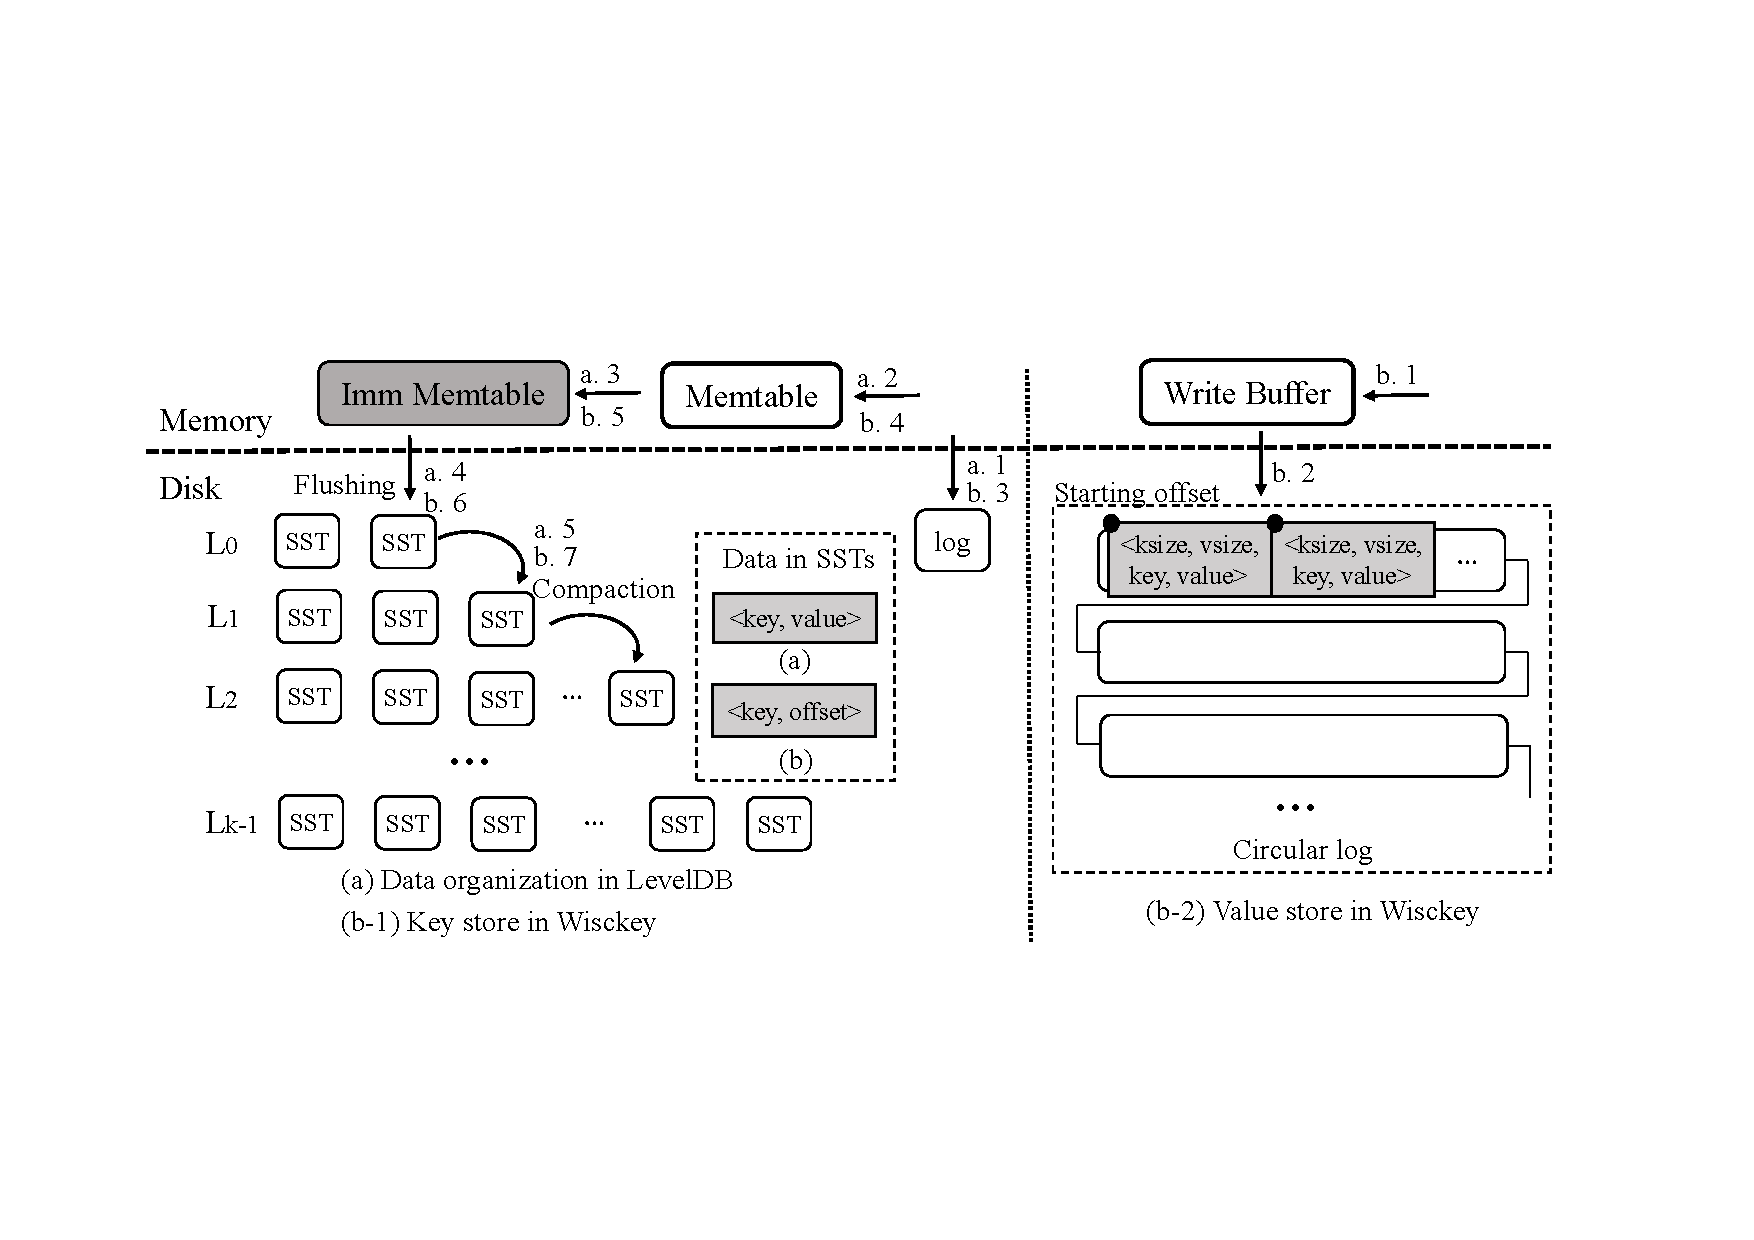
\includegraphics[width=80mm]{lsm_wisckey.pdf}}
	\caption{{\color{red}{The architecture of LevelDB (the part depicted with flag a) and Wisckey (the part depicted with flag b). LevelDB is used as a key store in Wisckey.}}}
	\label{fig::lsm_wisckey}
\end{figure}

%Wisckey的初衷是䌘化SSD侊LSM结构的KVstore的写攟倧问题然而由于GC匀销倧若是产生倧量的GC䌚造成Wisckey䞥重写攟倧并圱响写性胜
%对于操䜜读操䜜圚LSM䞭扟到offset圚LOG里面读出KV写操䜜先写vlog再将元数据曎新到LSM删陀操䜜盎接写到LSM
% operations to discard the invalid KV pairs and release the space
\paragraph{Wisckey} Wisckey is an SSD-conscious persistent KV store derived from LevelDB, which separates keys from values to significantly mitigate the write amplification so as to improve the endurance of SSD. The separated keys are used as indexes of the values. {\color{red}{Fig.~\ref{fig::lsm_wisckey} also illustrates the data organization in Wisckey, which consists of a key store and a value store. The key store, as shown in Fig.~\ref{fig::lsm_wisckey} (b-1), is an LSM structured store called the LSM-tree, e.g., LevelDB which is briefly introduced above. The value store, as shown in Fig.~\ref{fig::lsm_wisckey} (b-2), also includes a memory component and a disk component. The memory component is a write buffer, used to avoid the noticeable overhead caused by a large number of small writes to a file system, especially on a fast storage device for a write-intensive workload \cite{Arrakis, Wisckey}. The disk component is an append-only circular log called vLog. As shown in Fig.~\ref{fig::lsm_wisckey}, when writing a KV pair, first append it to the write buffer (b.1). When the buffer size exceeds its target size, it is flushed to vLog in the form of tuple \textless key size, value size, key, value\textgreater{} (b.2). Then bulk insert the keys along with the values’ info \textless vLog-offset, value-size\textgreater{} into the LSM-tree, which starts from the step (b.3), and the subsequent operations are as described above.}} When conducting a point lookup, it first queries the key in the LSM-tree as described in the preceding paragraph. If the key is found in the LSM tree, it returns the value info containing the vLog-offset which is then used to obtain the actual value from the vLog. In Wisckey, when the data volume in the vLog accumulates to a threshold size, it starts to trigger garbage collection (GC) to free space in the vLog and consolidate valid values (not overwritten or deleted) in a contiguous range of the vLog. Wisckey set two pointers to recognize the valid range of vLog: (1) the \textit{head}, where new values are appended; (2) the \textit{tail}, where to reclaim space by GC. The process of GC in WiscKey includes 1) read a chunk of key-value pairs (e.g., 64 MB) from the tail of the vLog, 2) check which of those values are valid by querying the LSM-tree, 3) rewrite valid values to the head of the vLog, and 4) free the space previously occupied by the chunk and update the tail accordingly. Therefore, the GC process involves reading and writing valid values, consuming a lot of computation and disk bandwidth resources.  In particular, real-world KV storage often exhibits strong locality \cite{Workload}, in which a small portion of KV pairs are frequently updated (i.e., hot data), while the remaining KV pairs receive only few or even no updates (i.e., cold data). Sequential GC order in vLog inevitably relocates cold data many times and unnecessarily increases GC overhead \cite{HashKV}.

\paragraph{HashKV} HashKV \cite{HashKV} is a KV separated store, aiming to mitigate the GC overhead under update-intensive workloads. The value store consists of vLog and reserved space. HashKV partitions vLog into fixed-size segments called main segment, and maps values into partitions in the vLog by hashing the associated keys. HashKV also partitions reserved space into segments called log segment, and allows a partition to grow dynamically beyond its size limit by allocating the KV pairs to reserved space. Thus, each partition includes one main segment and several log segments, called segment group. HashKV enables hot code data separation by storing cold KV pairs in a cold data block and applies GC to hot KV pairs to avoid re-copying cold KV pairs. In HashKV, GC is triggered when the free log segments in the reserved space are running out. The process of GC becomes 1) select a candidate segment group, 2) identify the valid KV pairs in the group, 3) write back the valid KV pairs to the main segment, or additional log segments if needed, in a log-structured manner, 4) release any unused log segments which can be later used by other segment groups and 5) update the latest value locations in the LSM-tree. HashKV sequentially scans the KV pairs in the segment group to identify the valid KV pairs (i.e., the KV pairs of the latest version) without querying the LSM-tree, thus significantly mitigating the GC overhead. Due to the  hotness awareness, HashKV mitigates write amplification and improves write performance.

%实验结果leveldb, wisckey从没有这些操䜜和频繁的操䜜所产生的写吞吐量和敎䜓写入量诎明写攟倧和写性胜问题
% and HashKV \cite{HashKV},HashKV builds atop KV separation and uses hash-based data grouping to map from values to storage space, combining with several design extensions to achieve both updates and GC efficient under update-intensive workloads. 
\paragraph{Impacts Compaction and GC} To quantitatively understand the impacts of GC on {\it{LevelDB}} (Version 1.20), {\it{Wisckey}} and {\it{HashKV}}, we have conducted a set of experiments on them, focusing on the impacts on write performance and write amplification. In the experiments, the KV size is 1 KB. We use single-threaded micro-benchmarks to evaluate the performance of LevelDB on 40 millions (M) writes using both sequential write (\textbf{SW}) and random write (\textbf{RW}). We leverage the testbed in HashKV \cite{HashKV} to evaluate Wisckey and HashKV on 40 M random writes (\textbf{Load}) and 12 M updates (\textbf{Update}), which triggers about (39 GB, 1.9 GB) and (12 GB, 0.78 GB) writes to vLog and the LSM-tree, respectively. 
%For LevelDB, the Memtable size is of 32 MB and the SST size is of 16 MB.  For Wisckey, the capacity of vLog is of 42 GB and the size of data chunk in each GC is of 64 MB.  

We configure the main parameters of three systems as follows:
\begin{itemize}
	\item LevelDB: Memtable size (32 MB), SST size (16 MB); 
	\item Wisckey: vLog capacity (42 GB), GC unit (64 MB); 
	\item HashKV: vLog capacity (40 GB), reserved space (2 GB), GC unit (segment group).
\end{itemize}

%The experimental results are shown in Table \ref{table:mo}. \textbf{WT}, \textbf{TW}, \textbf{C} and \textbf{GC} stand for write throughput, total write (represented in form of "vLog + LSM-tree" for KV separation stores), the number of compaction and the amount of GC, respectively.

The experimental results are shown in Table \ref{table:mo}. \textbf{WT}, \textbf{TW}, \textbf{C} and \textbf{GC} stand for write throughput, total write, {\color{red}{the number of compaction in the LSM-tree and the number of GC in the vLog}}, respectively. For KV separated stores, the total write is represented as the writes in (vLog, LSM-tree). Note that, Wisckey and HashKV start to trigger GC in update phase. As shown in Table \ref{table:mo}, LevelDB provides excellent write performance for sequential writes. However, for random writes which generate large amounts of compactions, the write throughput (WT) is significantly decreased, and the write amplification (WA) factor is more than 12X. For KV separated stores, in load phase, Wisckey has the best WT for random writes and no data rewrites in the vLog, but it suffers from 8X WA in the LSM-tree because of compactions; WT of HashKV is worse because of the complex segment management, WA in the LSM-tree is more than 13 X, and the reason of the difference with that in Wisckey is that the sequence of keys inserted to the LSM-tree is different.
% 芁改LevelDB RW............
\begin{table}[!t]
	\setlength{\abovecaptionskip}{0.cm}	
	\setlength{\belowcaptionskip}{-0.cm}
	\centering
	\caption{The negative impact of compaction and GC on write performance and write amplification. }
	\label{table:mo}
	\scalebox{0.8}{	
	\begin{tabular}{ccccccc}
			\toprule
			\multirow{2}{*}{\textbf{Metrics}} & \multicolumn{2}{c}{\textbf{LevelDB}} & \multicolumn{2}{c}{\textbf{Wisckey}} & \multicolumn{2}{c}{\textbf{HashKV}} \\
			\cmidrule(lr){2-3} \cmidrule(lr){4-5} \cmidrule(lr){6-7}
			& SW &  RW &  Load & Update & Load & Update \\
			\midrule
			WT (MB/s) & 77.1 & 7.0 &  103.4 & 8.6 & 63.9 & 11.9 \\
			TW (GB) & 39 & 475 & (39, 17) &  (29, 78) & (39, 26) & (64, 43) \\
			C & - & 6466 & 1563 & 4536 & 2109 & 4329 \\
			GC & - & - & - & 103 & - & 879 \\
			\bottomrule
	\end{tabular}
	}
\end{table}

%leads to an order of magnitude write amplification problem
%根据结果分析compaction对LSM-based KV store的性胜圱响曎新密集型应甚对Wisckey的圱响hashkv,wisckey的写性胜和总䜓写å…
As GC starts to be triggered in update phase, the number of GC in HashKV is much more than that in Wisckey, resulting in worse WA of HashKV in the vLog. The WT of both HashKV and WiscKey severely decreases, while the WT of HashKV stays better than that of WiscKey because of its optimized GC strategy. Overall, both HashKV and WiscKey generate severe WA in the LSM-tree because of large numbers of compaction. 

{\color{red}{Table \ref{table:mo} illustrates that in the LSM-tree, compaction has a significant negative impact on write throughput and write amplification. KV separation mitigates this problem for the whole store. However, the costly GC in Wisckey decreases the write throughput. Especially under update-intensive workloads, frequent GC in Wisckey arouses large amounts of cold data rewrites which results in more updates to the LSM-tree. HashKV presents a light GC to mitigate these problems under update-intensive workloads, but the complex segment management results in management overhead and a lot of system calls, which also harms the write throughput. In KV separated stores, the KV pairs discarded during the compaction process in the LSM-tree include the offsets of the stale values in the vLog. Take this into consideration, we attempt to figure out a method to mitigate the problem of write performance degradation.}}
%The difference on total write between them may result from the various insert sequence of keys. 

%and more than 2X write amplification in vLog. In the LSM-tree, it generates large amounts of compaction and more than 100X write amplification. 

%HashKV has lower write performance than Wisckey in the load phase because of its complex segment management. In the update phase, HashKV arouses more GC operations, resulting in more than 5X write amplification in vLog, but the optimized GC makes the write performance more efficient. Although it generates more compaction in the LSM-tree, the write amplification is lower than Wisckey because of the different data distribution. We observe that in the update phase, the size of vLog increases to 44GB in Wisckey, while the capacity of HashKV keeps below 42GB.

%分䞺讟计䞎实现䞀倧郚分
\section{Design and Implementation} \label{design}
This section presents our block manager, \textbf{B}lock-conscious \textbf{I}n-place reused log (BILog) and a new key-value (KV) separated store (BIKV). The overarching goal is to design a lightweight GC strategy so as to mitigate the write amplification and improve the write performance under GC-intensive workloads. In the following, we describe the basic design and detailed implementation of BILog and BIKV.

% Potential issues: 
% 1. how to remedy the random write (instead of append write) 
% 2. 
\subsection{Overall Design} \label{bd}
%捕获倱效offset,圓数据量蟟到阈倌时重甚倱效䜍眮
As discussed previously, in KV separated stores, when flushing the write buffer to the vLog, they first write the KV pairs to the given start offset in the vLog in the form of tuple \textless key size, value size, key, value\textgreater, then combine the keys and the value's info \textless vLog-offset, value-size\textgreater{} as KV pairs, and finally insert these KV pairs into the LSM-tree. In the LSM-tree, compactions happen frequently. During the compaction process, the LSM-tree discards stale KV pairs which include the starting offsets of the stale values in the vLog based on the fact that the LSM-tree only contains the currently valid values in the vLog. The currently employed garbage collection process in key value separated stores first scans a segment in the vlog and then rewrites the valid values. It reclaims space in a segment granularity. We observe that when key value pairs are invalidated and their new values are appended to the log, their previously occupied space in the log can be reused immediately.  A naive way to reuse the invalid value space is to obtain the starting offsets of the stale values in the vLog (called invalid offset) from the discarded KV pairs in the LSM-tree and record them in a buffer. To serve incoming data, it chooses an offset from the buffer and uses the offset as the starting point to write the data to the vLog. This method would incur a large amount of accesses to the file system. Especially, if the KV pair size is less than or not aligned with the SSD page size (e.g., 4KB), it causes severe fragmentation and has to run in asynchronous mode which compromises the durability of the KV store for improved endurance of SSD.
%简单的做法及存圚的问题由于倱效䜍眮重甚䌚造成随机写因歀方法蟃适甚于SSD倱效䜍眮重甚富臎频繁随机IO,解决方案是以块䞺单䜍管理recovery解决方案是倱效块状态持久化版本管理
%A naive way to reuse the invalid offsets is to simply write new KV pairs to the place of invalid offsets in vLog. However, there are several considerations, as follows:
%and transform the conventional circular vLog to 

To better achieve utilizing the invalid offsets and remedy the above problems, we build a block manager to record the invalid offsets in blocks, manage the blocks and assist in recycling invalid blocks ( Section \ref{ss1}). Based on the block manager, we design a block-conscious in-place reused vLog ( Section \ref{ss2}) and a lightweight GC strategy ( Section \ref{ss3}). We store the valid KV pairs found during a GC process (which we consider as \textit{cold data}) to a separate region in the vLog called \textit{reserved space} to isolate hot/cold data (Section \ref{ss2}). The metadata of blocks which identify the invalid offsets in the block manager can be persisted in an append-only log to recover the KV store in case of crashes as discussed in Section \ref{ss4}. 
%.  We use an append-only log to record the states of blocks, called block state log

We implement BIKV based on  the design of Wisckey. Fig.~\ref{fig:bikv} demonstrates the overall architectural view of BIKV.  As it is illustrated, BIKV consists of a key store, a block manager, and a value store. The key store is an LSM-tree structured KV store as it is with LevelDB. The in memory block manager gathers invalid offsets from the compaction process in the LSM-tree and assists block recycling in the GC process in the vLog. The metadata of blocks in the block manager is persisted in a block state log. The value store includes a write buffer whose size is an integer multiple of the block size and a recycled vLog implemented as BILog based on the block manager. We provide detailed descriptions of the implementation of BIKV in the following.

%The memory component in BIKV consists of the write buffer for new KV pairs and our new block manager.  For the disk component, the key store is an LSM-tree structured KV sotre (e.g., LevelDB default), and the value store is a recycled value log implemented as BILog based on the block manager.  We persist the states of blocks in the block manager to a 

%架构囟
\begin{figure}[!t]
	\setlength{\abovecaptionskip}{0.cm}	
	\setlength{\belowcaptionskip}{-0.cm}
	\centerline{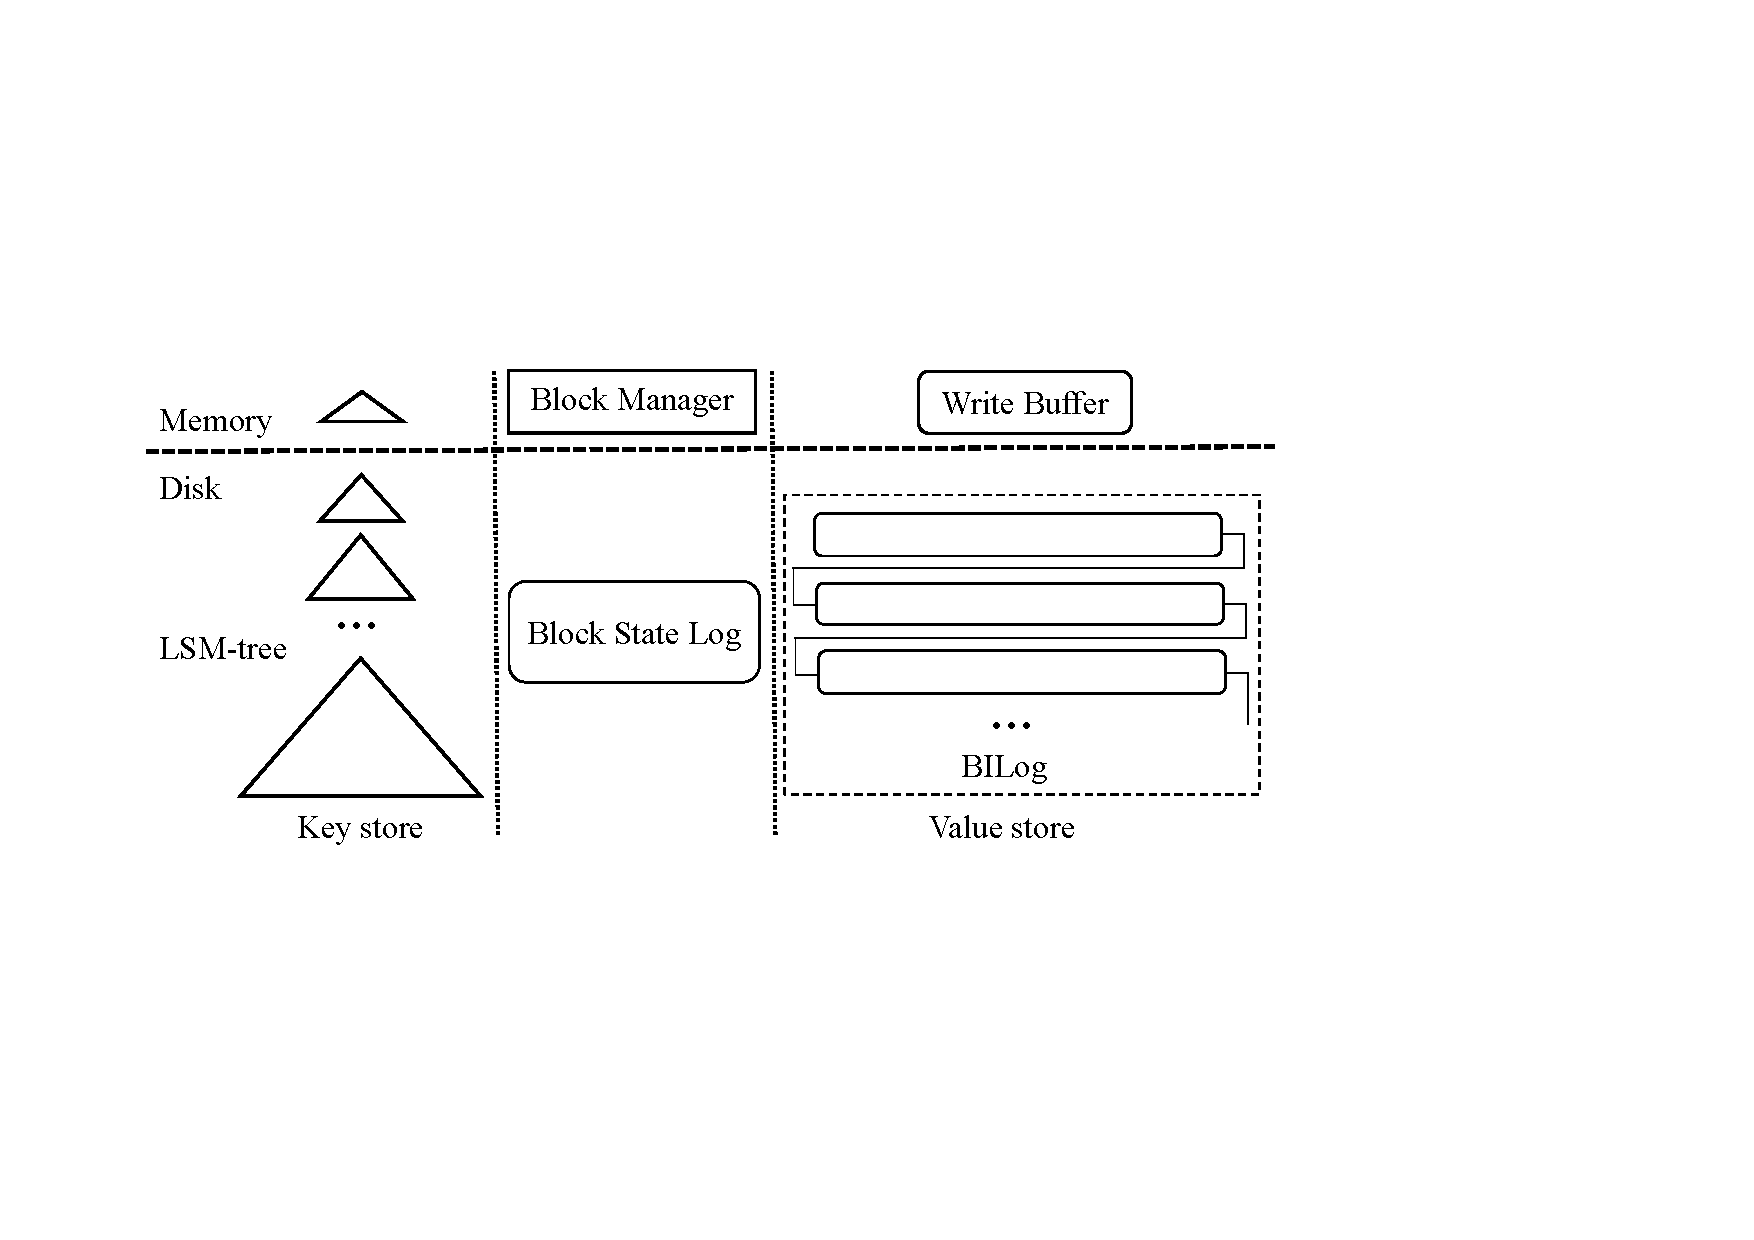
\includegraphics[width=90mm]{bikv.pdf}}
	\caption{The overall architectural view of BIKV. BIKV incorporates a block manager which collects the information about the offsets of invalid values and facilitates reusing the space without waiting until garbage collection is triggered. }
	\label{fig:bikv}
\end{figure}

%倱效块管理
\subsection{Block Manager} \label{ss1}
%数据结构2种倱效offset版本控制策略频繁GC和update前提䞋倱效offset版本控制和普通莟蜜䞋
%块粒床
%倱效块和有效块
%细节暡块的实现以及实验䞭遇到的问题对于曎新密集或非密集情况䞋重甚块状态的管理
We build a block manager to record the validity of KV pairs in blocks, which covers the whole storage space of the vLog. Initially, all KV pairs are valid. As compactions in the LSM-tree occur, the block manager continuously collects the invalid offsets of the discarded KV pairs during the compaction processes. In this section, we introduce the detailed implementation of the block manager.
%For update-intensive workloads, it discards a large number of stale KV pairs during a compaction process in the LSM-tree of KV separation stores. The value of the discarded KV pairs is the offset of the stale values in the vLog. We build an invalid block manager to collect the invalid offsets, manage them in blocks (a block that contains invalid offsets called an invalid block, otherwise is a valid block) and reuse the invalid blocks in batches.

\subsubsection{Block Granularity}
%防止SSD的碎片化对霐4KB选择KV size和4KB的最小公倍数***************管理粒床的描述需芁再斟酌䞀䞋
%In this paper, we focus on observing the benefits of the in-place reusable vLog for the KV stores that separate keys from values under update-intensive workloads. Thus, we assume the size of KV pairs remains constant.
The first step of building the block manager is to determine the block size $BS$, which is the management granularity of the block manager. We align the block size to SSD page size to eliminate the fragmentation of SSD. Thus, we set the block size as the common multiple of SSD page size and KV size to align both the size of the SSD page and KV pair. For example, if SSD page size is of 4 KB and KV pair size is of 1 KB, the block size is set as 4 KB. 

\subsubsection{Offset State in the vLog}
%数据结构包括2䞪状态䜍囟衚瀺块重甚前和重甚后状态
%因䞺各䞪偏移所对应的KV对只有2种状态有效或无效因歀对于每䞀䞪块䜿甚䜍囟来衚瀺块内所有䜍眮的状态。圚确定块倧小后讟计敎䞪VLOG的块数块内的偏移数来构建块管理噚
The block manager covers the whole storage space of the vLog $SS$. After determining the block size $BS$, we sequentially divide the vLog into segments in block granularity. The number of blocks $BN$ is calculated by dividing the storage space of vLog by the block size ($SS$/$BS$). We assume the KV pair size is fixed $KS$. Then, we acquire the number of KV pairs $KN$ in each segment by dividing the block size by the KV size ($BS$/$KS$), which means each block manages such number of offsets. We use the state of an offset to represent the state of the KV pair it mapped in the vLog in the following.

We should be careful about mitigating the memory cost of the block manager. We use two simple hashes to scale down the vLog space: 1) dividing the starting offset of a block by the block size as the new starting offset; and 2) executing modulo operation between an offset and the block size and dividing the result by the KV pair size as intra-block offset. Thus, a block consists of a starting offset and $KN$ intra-block offsets.
%The number of intra-block offsets in a block is .

There are only two states of the KV pairs in the vLog: valid or invalid, which means we can use the \textit{bool} type to identify the validity of KV pairs. Thus, we use the \textit{bitmap} for each block to record the state of the offsets that belong to the block, represented as \textit{vLog-offset\_s}. The length of a bitmap is $KN$. We use 0 (default value) as valid flag, and 1 as invalid flag. When collecting an invalid offset, we compute the starting offset to locate the block to which the offset belongs, and compute the intra-block offset to mark the corresponded bit position in \textit{vLog-offset\_s} to 1. When finishing the recycling of a block in a GC process, we clear \textit{vLog-offset\_s} of the block and mark all positions to 0. When recycling a block, we only need to verify the validity of KV pairs at the offsets with a valid flag in \textit{vLog-offset\_s} of the block.

\subsubsection{Offset State in the LSM-tree}
The way of identifying the validity of KV pairs is the same as that in Wisckey. For an offset with the valid flag in \textit{vLog-offset\_s}, it queries the key and extracts the offset from the value in the LSM-tree. And then it compares the two offsets. If they are the same, it indicates the KV pair is valid, otherwise, the KV pair is invalid. When recycling a block, after identifying the validity of the offsets, the subsequent processes vary based on the validity:
\begin{itemize}
	\item For an invalid offset, it means that the stale index in the LSM-tree has not been discarded. When reusing this block, we write a new KV pair at the offset in the vLog and insert an index with the new key to the LSM-tree. 
	\item For a valid offset, we rewrite the KV pair to the vLog and insert an index with the new offset to the LSM-tree, resulting in that the former index in the LSM-tree becomes stale. 
\end{itemize}
%If an offset is verified to be invalid If an offset is verified to be valid, we rewrite the KV pair to the vLog and insert a KV pair with the new offset to the LSM-tree, resulting in that the former KV pair in the LSM-tree becomes stale. 
%The two situations both indicate that

In either of the above two cases, the offset is emerged twice or even more at the same time in the LSM-tree, which causes consistency problem: when the stale version of the offset is discarded in the LSM-tree, it marks the offset as invalid; but actually, currently the KV pair at that offset is valid. If the block is recycled later, it results in data loss within the block. In other words, we can find the key in the LSM-tree, but the KV pair at the offset in the vLog does not match the key. To resolve this problem, we have to record the offsets which have multiple versions in the LSM-tree.

The frequency of compaction in the LSM-tree and of GC in the vLog affect the existence of offset versions. We first assume there are at most two versions of an offset in the LSM-tree. Thus, we use another bitmap for each block to record the states of offsets in the LSM-tree, represented as \textit{LSM-offset\_s}. Similarly, 0 (default value) represents a valid flag (i.e., only one version), and 1 represents an invalid flag (i.e., existing two versions of the offset). When recycling a block in a GC process, for the positions with a valid flag in \textit{vLog-offset\_s} of the block, we mark the same bit positions to 1 in \textit{LSM-offset\_s}. When collecting an invalid offset which has an invalid flag in \textit{LSM-offset\_s} of the block it belongs to, we discard the offset directly and mark the bit position to 0.

%重新画囟4䜍䞺䟋2䞪阶段GC前GC后
%In summary, the data structure of the states of a block (ie, the metadata) in the block manager consists of two bitmaps, representing the state of offsets in the vLog and the LSM-tree, respectively. 
To better understand the block states, Fig.~\ref{fig:iblock} gives an example of the two state bitmaps of a block. The length of the bitmap is 4. Before recycling the block, \textit{vLog-offset\_s} of the block accumulates 3 invalid flags, and only the first offset is valid, while the states in \textit{LSM-offset\_s} are all valid. When recycling the block in a GC process, the states in \textit{vLog-offset\_s} facilitate realizing a lightweight GC. After finishing the recycling of the block, correspondingly, the first position in \textit{LSM-offset\_s} is set as 1, while \textit{vLog-offset\_s} is cleared and the states are set as 0. The memory cost of the two bitmaps is negligible with 2 bits for each offset. For a vLog containing 1 billion offsets, the memory cost is about 239 MB.

%12.9 36MB的曎新标泚zifian分垃
It should be noted that we have performed extensive experiments to effectiveness of \textit{LSM-offset\_s} for the consistency problem resulting from the multi-version offsets in the LSM-tree. We find that under update-intensive workloads when it triggers GC intensively, there exists a situation that some blocks are frequently reused, {\color{red}{which is aroused by the higher compaction priority of hot data in the LSM-tree (i.e., the compaction requirement of $L_0$ is determined by the number of SSTs)}}. It results in a few multi-version offsets in the LSM-tree causing data loss. For example, in an experiment using 1 KB-KV pair and 4 KB-block with 40 M inserts, 36 M updates following a heavy-tailed Zipf distribution and 40 M reads in order, it generates several three-version offsets and results in 70 KV pairs lost. In this case, we change the bool state to counting state, which guarantees the consistency but costs more memory. {\color{red}{When the bock size increases to 8 KB or even larger, using \textit{LSM-offset\_s} can guarantee consistency}}. {\color{red}{Under this workload, we also find that when the bock size increases to 8 KB or even larger, using \textit{LSM-offset\_s} can guarantee consistency. It is attributed to the number of offsets a block contains, less number of offsets raise up the probability to be frequently reclaimed and reused.}}
%the less the number of offsets, the more probabilty to be frequently reclaimed and reused

%倱效块状态囟
%Invalid status tables for each block in Invalid Block Manager
\begin{figure}[!t]
	\setlength{\abovecaptionskip}{0.cm}	
	\setlength{\belowcaptionskip}{-0.cm}
	\centerline{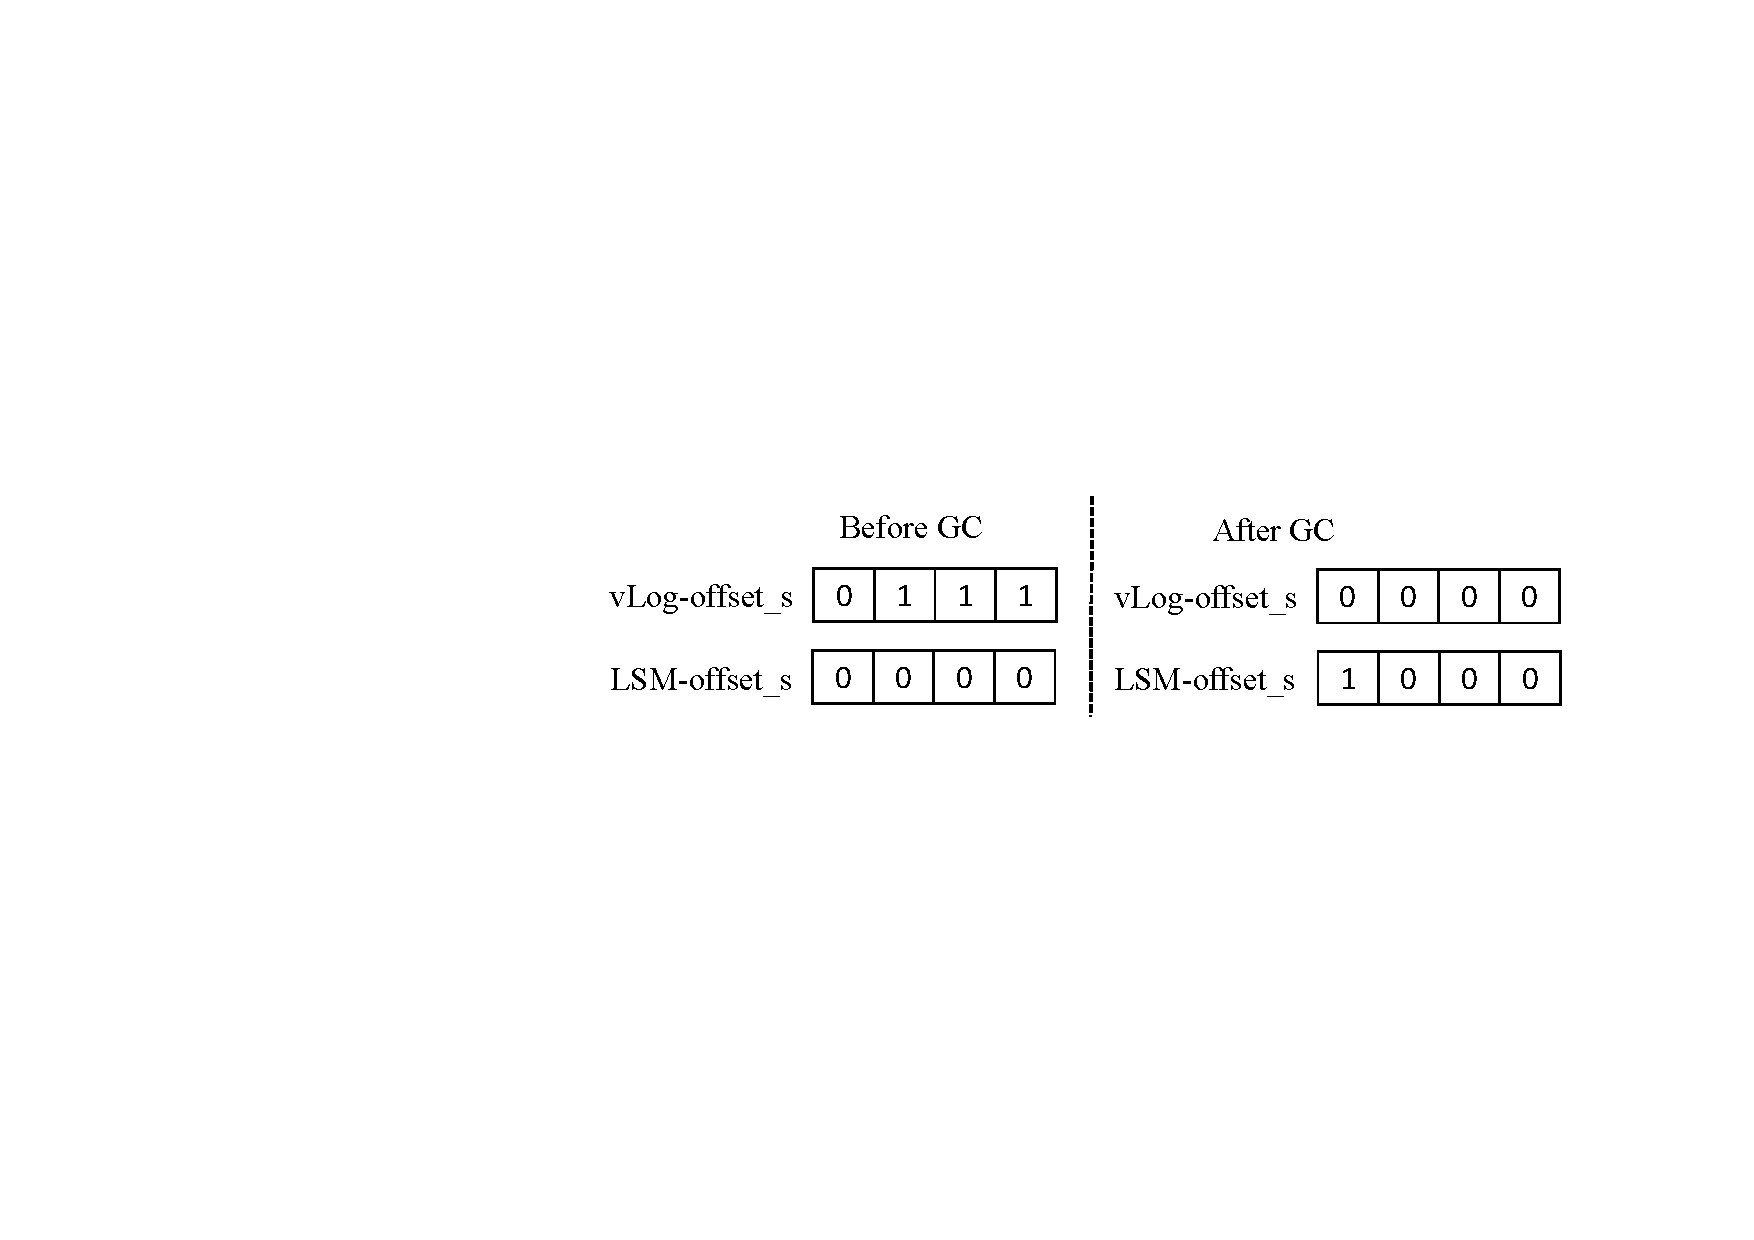
\includegraphics[width=80mm]{bitmap.pdf}}
	\caption{An example of two state bitmaps of a block. {\color{red}{Before GC, \textit{vLog-offset\_s} accumulates invalid offsets in the vLog, after GC,  \textit{vLog-offset\_s} is cleared and\textit{LSM-offset\_s} records the multi-version offsets existed in the LSM-tree.}}}
	\label{fig:iblock}
\end{figure}

\subsubsection{Block Classification}
As invalid offsets accumulate over time, there exist three types of blocks based on the states in \textit{vLog-offset\_s} of a block, which have individual recycling processes, as follows: 
\begin{itemize}
	\item Entirely invalid block: the states are all invalid. When recycling this type of block, it directly clears the states in \textit{vLog-offset\_s} of the block.
	\item Partially Invalid block: part of the states are invalid. When recycling a partially invalid block, it first verifies the validity of the KV pairs according to the valid flags in \textit{vLog-offset\_s} and marks these positions in \textit{LSM-offset\_s} as 1. It then rewrites the valid KV pairs to the vLog and inserts the indexes to the LSM-tree. Finally, it clears the states in \textit{vLog-offset\_s} and set them as 0.
	\item Valid block: the states are all valid. Such blocks are exempt from being recycled.
\end{itemize}

In BIKV, we employ a priority policy when recycling the blocks based on the states in \textit{vLog-offset\_s} of each block, i.e., entirely invalid block $>$ invalid blocks with more than half invalid flags (called half invalid block) $>$ other invalid blocks. This specification minimizes data rewrites and reduces the number of point queries in the LSM-tree, but meanwhile it probably results in large amounts of access to the vLog. The blocks with high priority are usually less and probably distribute randomly. Thus, we buffer the starting offsets of the entirely invalid blocks and half invalid blocks in sorted order to save the iterating time for locating them and reduce accesses to the vLog at the cost of memory space, represented as \textit{buffer\_eib} and \textit{buffer\_hib}, respectively. For the invalid blocks, we set a pointer $pointer\_ib$ to loop the whole blocks in the block manager.

Generally, the GC unit size is larger than the write buffer size. Thus, we also buffer the starting offsets of the blocks recycled in a GC operation, represented as \textit{buffer\_rb}. For the entirely invalid blocks, it directly inserts them in \textit{buffer\_rb} when it triggers a GC operation. The memory cost of these buffers is negligible and varies under different block sizes and KV pair sizes. 

\subsubsection{Block State Log}
%甚猖码和解码的方匏持久化状态或盎接按01持久化
We persist the states in \textit{vLog-offset\_s} and \textit{LSM-offset\_s} of blocks in the block manager to the block state log, aiming to recover the KV store and the indices not inserted into the LSM-tree during a GC operation in the event of a crash. The states of blocks are changed by three operations: compaction in the LSM-tree, GC in the vLog, and reusing available blocks. During a compaction operation, the block manager collects the invalid offsets from the values of the discarded KV pairs in the LSM-tree, and the states in \textit{vLog-offset\_s} of some blocks are changed. In a GC operation, the states in \textit{LSM-offset\_s} of the recycled blocks are modified. When reusing the blocks in \textit{buffer\_rb}, the states in \textit{vLog-offset\_s} of these blocks are set as 0. 
%Thus, after finishing these operations, we persist the states in the corresponding bitmap of the blocks to the block state log.  

%We design a priority to select the candidate blocks in a GC operation based on the states in \textit{vLog-offset\_s} of each block
%Each block is mapping to a continuous segment in vLog. The data structure of each block consists of the starting offset (i.e., )
%The size of the offsets extracted from the KV pairs in the LSM-tree is 8 B. 
%locate the block and intra-block location according to a invalid offset  
%块重甚
\subsection{Implementation of BILog} \label{ss2}
%倱效块状态党倱效和郚分倱效党倱效块䞻劚重甚郚分倱效块被劚重甚,半倱效块重甚时需芁GC
%讟计冷热区域vlog预留郚分写入GC数据䞻区域写入后续的新数据
%数据flush时路埄选择算法
%flush数据䜍眮选择噚写䞪算法:䞻劚重甚和被劚重甚
%新BILog的capacity是觊发GC的容量指热数据的胜力䌚预留䞀些空闎攟GC后的冷数据预留空闎䞍足时把数据写入热区域
Based on the block manager, we design a block-conscious in-place reused vLog (BILog). We reclaim the space of vLog in blocks. When flushing the write buffer, we write the KV pairs to several blocks sequentially or randomly according to the available blocks, i.e., sequential write before starting to trigger GC and sequential/random write on recycled blocks. Generally, the size of valid KV pairs left in a GC process (which we consider as \textit{cold data}) is not aligned with the block size. To eliminate the block fragmentations, we write the valid KV pairs to a separate region in the vLog called \textit{reserved space}, which meanwhile realizes the separation of hot/cold data. Thus, the storage space of the vLog is divided into two parts: a large piece for new data and a small piece for cold data, called main space and reserved space, respectively. We call the size of the main space as the capacity of vLog. When the data volume accumulates to the capacity of vLog, BIKV starts to trigger GC.

In BIKV, the valid range of vLog is always from 0 to the \textit{tail} (i.e., the pointer points to the current end of the vLog). The new data is always appended at the tail. Before thoroughly filling the main space, the new KV pairs are appended at the tail in the main space. After that, the valid KV pairs during GC operations are appended at the tail in the reserved space. Whenever the position of the tail changes, we insert the tail and its offset into the LSM-tree in the form of tuple \textless `tail', offset \textgreater. Fig.~\ref{fig:ipbrLog} illustratively shows the data organization in BILog. The shadow positions indicate the invalid values, and the dotted box represents the data range of a block. The tail points to a position in the reserved space. Before that, the vLog is filled with KV pairs.  
%the reclaiming invalid blocks 

\begin{figure}[!t]
	\setlength{\abovecaptionskip}{0.cm}	
	\setlength{\belowcaptionskip}{-0.cm}
	\centerline{\includegraphics[width=80mm]{vLog.pdf}}
	\caption{Data organization in BILog. {\color{red}{The storage space is divided into blocks (dotted box). The main space is used to store hot data, while the reserved space is used to store cold data. The data is appended to the tail, the filled space performs in-place update.}}}
	\label{fig:ipbrLog}
\end{figure}

\subsection{Garbage Collection} \label{ss3}
%圓BILog环积到阈倌倧小时就匀始觊发GC匀始觊发GC后根据可甚块池䞭的块的倧小是吊倧于buffser size来决定芁䞍芁GCGC单䜍是块倧小和写猓冲的公倍数
Garbage collection is indispensable to reclaim the space occupied by invalid values in the vLog. In BIKV, GC operates in units of an integer multiple of block size $GC_u$ (e.g., 64 MB), and is triggered when the capacity of vLog is running out. We design a lightweight GC strategy with the aid of the block manager, and overall, a GC operation is to recycle the blocks with invalid flags. The number of blocks recycled in each GC $GC_bn$ is determined by dividing the GC unit size by the block size.

In BIKV, if it finds that the tail is at the end of the main space or moved to the reserved space when flushing the write buffer, it starts to trigger GC. At the beginning of GC, we poll the blocks according to the priority to select the candidate blocks and then recycle these blocks. The process is shown in Algorithm~\ref{alg:gc}.
%GC策略写䞀䞪算法 
%When it starts to trigger GC, if the total size of the entirely invalid blocks is more than the GC unit size (e.g., 64 MB default), we directly clear the states in \textit{vLog-offset\_s} of these blocks and flush the KV pairs in the write buffer to these blocks subsequently. If the entirely invalid blocks are running out (i.e., the size of the left blocks is less than GC unit size), it starts to recycle the blocks.
\begin{algorithm}[htbp]
	\caption{The process of a GC operation}
		\begin{algorithmic}[1]
			\IF{There exists entirely invalid blocks}
			\STATE Insert the blocks in \textit{buffer\_eib} to \textit{buffer\_rb}; 
			\ENDIF
			\IF{The total size of the blocks in reusable block pool is larger than the write buffer size} 
			\STATE Skip;
			\ELSE
			\IF{There exists half invalid blocks} 				
			\IF{The total size of these blocks is larger than GC unit size}
			\STATE Get $GC_bn$ blocks from \textit{buffer\_hib};
			\ELSE
			\STATE Get all half invalid blocks from \textit{buffer\_hib};  
			\STATE Get the remaining number of invalid blocks by looping the block manager with $pointer\_ib$;
			\ENDIF
			\ENDIF
			\STATE Reclaim the candidate blocks and insert them to \textit{buffer\_rb};
			\ENDIF
		\end{algorithmic}
	\label{alg:gc}
\end{algorithm}

After finishing the GC operation, we flush the write buffer to the available blocks in \textit{buffer\_rb}. Overall, when flushing the write buffer to the vLog, we should select the write location according to the tail. The algorithm of the write location selection for flushing is shown in Algorithm~\ref{alg:reuse}. When the write buffer is full, it flushes the data to the vLog. The first step is to decide the position of the tail. If the tail is in the main space, it directly appends data to the tail of vLog. Otherwise, it determines whether to trigger a GC operation based on the number of blocks in \textit{buffer\_rb}. 

\begin{algorithm}[htbp]
	\caption{Write location selection algorithm for flushing}
	\begin{algorithmic}[1]
		\STATE Get the tail of vLog; 
		\IF{The tail is in the main space} 
		\STATE Append data to the tail of the vLog;
		\ELSE
		\IF{The total size of blocks in \textit{buffer\_rb} is more than the write buffer size}
		%\COMMENT{All values in the segments managed by those blocks are invalid} %测试
		\STATE In-place update data to these blocks and erase them from \textit{buffer\_rb};
		\ELSE
		\STATE Trigger a GC operation; 
		\STATE In-place update data to the available blocks and erase them from \textit{buffer\_rb};
		\ENDIF
		\ENDIF			
	\end{algorithmic}
	\label{alg:reuse}
\end{algorithm}
 
% This rule has a complex impact on GC overhead because it reduces the number of KV pairs which need to identify the validity (i.e., point queries) in the LSM-tree, but probably results in large amounts of access to the vLog.
%Based on the invalid block manager, we design two invalid block reuse policies: a positive reuse policy and a negative reuse policy. The positive reuse policy is to actively reclaim the entirely invalid blocks (i.e., the invalid offset bitmap of vLog in a block is all set to 1) before the size of vLog accumulating to a threshold, aiming to mitigate management overhead and save storage space. The positive reuse policy is triggered when flushing KV pairs in the write buffer to the vLog. The negative reuse policy is to passively reclaim the invalid blocks after the volume of values in vLog accumulating to a threshold. It is triggered in the process of garbage collection to discard the stale values and release storage space.
%When reusing a block, we iterate through the invalid offset bitmap of vLog, for the position whose value is 0, we query the LSM-tree to check the validity of the KV pair. If the offset is stale for that key in the LSM-tree, we set the corresponding position in the invalid offset bitmap of the LSM-tree to 1. 
%When the data in vLog accumulates to a threshold, it starts to trigger GC. The process of GC is lightweight with the help of the invalid block manager. First, based on the invalid offset bitmap of vLog in each block, acquire a specific volume of blocks (e.g., 64MB) in which the number of invalid offsets accounts more than others. Second, read the KV pairs in those blocks except the entirely invalid blocks. Third, find which of those values that corresponding bit position are 0 are valid by querying the LSM-tree. Finally, append valid values back to the vLog and modify the invalid offset bitmap of vLog in these invalid blocks to be 0. Subsequently, we flush new data to the GCed invalid blocks. 

%\subsection{In-place Block Reusable vLog}
%对于被劚重甚的操䜜我们将vlog分䞺可甚郚分和预留郚分䞻芁有2䞪奜倄解决被劚重甚䞭有效数据的写对霐问题将GC后的有效数据盞对冷数据写到预留䜍眮劂囟所瀺
%In IpBrKV, the value log is an in-place reuse vLog. Since the vLog is recycled based on blocks, we call it in-place block-reusable vLog. For the negative reuse in IpBrKV, it triggers GC operations, resulting in valid data in the reclaiming invalid blocks be rewritten. To simplify the block management, we divide the vLog into available part and reserved part. The new data is always written into the available part; while the valid data produced in GC operations is rewritten into the reserved part. There are two benefits to this distribution: (1) avoid the problem of write alignment caused by rewriting the valid data into the reusable blocks; (2) realize separation of hot and cold data, because the valid values rewritten in GC operation are relatively cold data. There is an example of the data status of the two parts in in-place block-reusable vLog, as shown in Fig.~\ref{fig::ipbrLog}. The shadow positions indicate the invalid values, the Dotted box represents the data range that a block maps to.

\subsection{Recovery} \label{ss4}
%基于Wisckey的foundation拥有其盞关的䞀臎性方案劂容忍猓冲数据䞢倱key store的䞀臎性由于采甚就地块重甚技术因歀将writefront和in-place update block offset持久化到LSM-tree同时䞺了支持可恢倍添加倱效块状态日志就劂同LevelDB侭的version的持久化䞀般持久化倱效块状态每次compaction后持久化圓前倱效块管理噚䞭存圚倱效偏移量的各倱效块状态
%
The recovery methods of BIKV are different from those of Wisckey because of BILog. If there happens a crash, the recovery process of the indices in the key store includes two steps. First is the recovery in the LSM-tree, i.e., scanning the write-ahead log after reboot to recover unpersisted KV pairs. Second is the recovery of the bulk indices not inserted into the LSM-tree during flushing the write buffer or GC in the vLog, i.e., getting the offset of the tail from the LSM-tree and scanning the vLog starting from the offset. If there exists data, get the key and offset, and keep forward scanning till the end, finally insert the indices to the LSM-tree. Otherwise, getting the offset of the last inserted non-tail key from the LSM-tree, scanning the block state log until finding the block that offset belongs to, and keeping scanning to get the offset of the reused blocks till the end, finally inserting the indices of the KV pairs in those blocks to the LSM-tree. It is necessary to recover the states of blocks in the block manager. Otherwise, BIKV degenerates to Wisckey at initially recovered until accumulating a number of invalid offsets. We recover the states by scanning the block state log till the end.

%\subsection{Limitations}
%由于是就地曎新因歀应甚场景有纊束适甚于固定KV倧小的应甚或倧郚分倧小盞近䌚产生少量的空闎浪莹,本文䞭的实验䜿甚固定的KV进行对可变KV倧小的支持可后续研究
%KV size,蟃坏情况䞋倱效的块䞍连续面䞎着产生倧量随机读写的问题圚SSD䞋随机读写和顺序性胜盞关䞍倧䜆是IO次数变倚仍然䌚有圱响
%In summary, there are several limitations for the block-conscious in-plate update
%In a worse case that the invalid blocks are discontinuous, it results in large amounts of random reads and writes. Although the difference between the sequential and random performance is not significant, the large number of I/Os has a negative impact on the system. 
%Intuitively, the nature of in-place reuse makes BIKV not suitable for the applications in which the size of KV pair is variable. In this case, it makes the invalid block management more complicated and will result in a certain amount of space waste. In this paper, we focus on observing the benefits of the design of in-place reuse in blocks under update-intensive workloads. Thus, we assume the KV size remains fixed to simplify the design of the invalid block manager.

\section{Evaluation} \label{evaluation}
%写攟倧空闎攟倧写性胜读性胜
%䞍同倧小的KV pairs的写攟倧空闎攟倧写性胜读性胜
%Wisckeyhashkv的预留空闎䞍同(GC少)时䞉者的性胜
%LSM-tree䞭产生的compaction的数量分析compaction对写性胜的圱响建议采甚compaction䌘化的LSM-tree
%就地曎新所产生的随机写圚HDD䞊的圱响
In this section, we conduct a set of experiments to evaluate BIKV and compare it against widely-used and state-of-the-art LSM structured and KV separated KV stores, including LevelDB \cite{LevelDB}, HyperLevelDB \cite{HyperLevelDB}, PebblesDB \cite{PebblesDB}, Wisckey \cite{Wisckey} (i.e., vLog implementation in the prototype of HashKV), HashKV \cite{HashKV} {\color{red}{and KVell \cite{KVell} (i.e., a KV separated store uses in-memory B tree as index)}}. We evaluate the KV separated stores with the testbed in HashKV which generates workloads using YCSB \cite{YCSB}, and evaluate LSM-based KV stores using the microbenchmarks (\textit{db\_bench}). For fair comparison, we replace the key generator in \textit{db\_bench} with that in the testbed to produce similar workloads. {\color{red}{We also modify the workload generator in KVell to produce the KV pairs under the same distribution with the testbed.}} The evaluation results attempt to answer the following questions:
\begin{itemize}
	\item How is the write and read performance of BIKV compared to other KV stores under mixed write/read workloads?
	\item How is the write amplification and performance of BIKV compared to other KV stores under GC-intensive workloads with varying KV pair sizes?
	\item What is the impact of GC strategies and the number of GCs on the {\color{red}{LSM-indexed}} KV separated stores under different GC timing?  
	\item What is the impact of the management granularity in BIKV?
\end{itemize}

\subsection{Experimental Setup}
%是吊甚䞀䞪衚衚明各KV store参数
The evaluation is performed on an Intel Xeon E5-2609v2 2.5 GHz processor with two cores, 32 GB of RAM, running 64-bit Centos 7.2 with the Linux 3.10 kernel. The xfs file system is run on top of a 480 GB SSD (ATA GALAX GXTA1C0480). 

\begin{table}[!t]
	\setlength{\abovecaptionskip}{0.cm}	
	\setlength{\belowcaptionskip}{-0.cm}
	\centering
	\renewcommand\tabcolsep{4pt}
	\renewcommand\arraystretch{1.1}
	\caption{Parameters of the six KV stores}
	\label{tab:p}
	\scalebox{0.8}{
		\begin{tabular}{cccccc}
			\hline
			 & \textbf{KV stores} & \textbf{MT} (MB) & \textbf{SST} (MB) & \textbf{BF} (b/k) & \textbf{GC unit} \\
			\hline
			 & \textbf{LDB} & 32 & (4,16,32) & 10 & -\\
			LSM & \textbf{HDB} & 32 & default & 10 & - \\
			structured & \textbf{PDB} & 32 & default & 10 & - \\
			\hline
			 & \textbf{Wisckey} & 4 & (2,4) & - & 64 MB\\
			KV & \textbf{HashKV} & 4 & (2,4) & - & segment group\\
			separated & \textbf{BIKV} & 4 & (2,4) & - & 64 MB \\
			\hline
		\end{tabular}
	}
\end{table}

%the six KV stores,
The major parameters of LevelDB (\textbf{LDB}), HyperLevelDB (\textbf{HDB}), PebblesDB (\textbf{PDB}), Wisckey, HashKV, and BIKV are shown in Table \ref{tab:p}. The larger size of Memtable can improve the write performance \cite{OHDB, FloDB}. The larger size of SST can improve the read performance \cite{OHDB}. In HashKV, a segment group includes a main segment (64 MB) and several log segments (1 MB). In LevelDB, the size of SST increases with the size of KV pairs. Besides, in the LSM structured stores, we turn off the data compression since there is no data compression in the KV separated stores. For other parameters, such as the threshold size of each level, we use the default values in the experiments. For the KV separated stores, we use LevelDB as the key store. The size of write buffer is set to 1 MB. We use the hotness awareness extension for HashKV which can improve the write performance and reduce write amplification. {\color{red}{For KVell, we do several experiments under various configurations and choose an experimental result which is relatively better at update performance and space amplification but slightly worse at write/read performance, configured with one disk, two workers and one load thread. KVell implements a producer-consumer like GC strategy, when deleting a KV pair, buffer its location and reuse it immediately when new data comes.}} The size of KV pairs is fixed, such as 1 KB, including the 8 bytes metadata (consisting of sequence number and type in LSM structured stores or key/value size in KV separated stores), 24 bytes key, and 992 bytes value. We use multi-step single-threaded micro-benchmarks to evaluate the write and read performance, performing 40 M inserts (about 39 GB of data, resulting in about 1.9 GB of key store in KV separated stores), four rounds of 12 M updates (about 12 GB of data, resulting in about 0.78 GB of key store) following a heavy-tailed Zipf distribution and two rounds of 40 M reads. The seven-step operation is Load, Update \#1, Update \#2, Read \#1, Update \#3, Read \#2, Update \#4 in turn. {\color{red}{Explain why we use these seven step? what are their respective purposes?}} {\color{red}{We follow the workload design of HashKV to stress-test the performance of the KV stores. We observe that large amounts of reads trigger  \textit{seek\_compaction}, which clears the space of lower levels and discards the stale KV pairs in the LSM-tree. Thus, we add two rounds random read to observe the read performance as well as the impact of intensive reads among writes-intensive workloads.}}
%In the load step, it performs 40 M random writes (about 39 GB of data, resulting in about 1.9 GB of key store in KV separation stores). In each update step, it performs 12 M updates (about 12 GB of data, resulting in about 0.78 GB of key store) following a heavy-tailed Zipf distribution. In each read step, it performs 40 M random reads.

\subsection{Performance Comparison}
%键倌分犻存傚䞭LSM-tree郚分采甚的是默讀参数的实验结果之后的实验䞭SST的倧小改䞺4MB
This section evaluates the write and read performance of the six KV stores. We use the default parameters of the LSM-tree in KV separated stores where the SST size is of 2 MB, while in other sections, we set the SST size as 4 MB to accelerate the experiments. We fix the size of each KV pair as 1 KB. In the experiments, we observe that after performing all the steps, the size of maximum space amplification of LevelDB, HyperLevelDB, PebblesDB {\color{red}{KVell}} is about 63 GB, 51 GB, 63 GB and 51 GB, respectively.  We set the capacity of Wisckey, HashKV and BIKV to be 58 GB (i.e., they all start to trigger GC when the size of vLog accumulates to 58 GB). In HashKV, we set the main segments 40 GB and the log segments 18 GB. 
% In HashKV, it starts to trigger GC when the reserved space is running out while Wisckey and BIKV start to trigger GC when they fills up the vLog.

The experimental results are shown in Fig.\ref{fig:pc}. We can observe the write performance of random write, intensive update and write after read, as well as the read performance. Note that the KV separated stores start to trigger GC in Update \#2.

\paragraph*{Random write}
%随机写基本没有或蟃少update 
In Load, it performs 40 M random writes. The write throughput of BIKV is close to Wisckey, and much better than the other four KV stores. In Update \#1, it performs 12 M updates immediately. The write throughput of Wisckey and BIKV are also better than others, but the benefits have reduced when compared to the Load phase, which is attributed to the compactions in the LSM-tree occurred during Update \#1. {\color{red}{The write throughput of KVell significantly degrades caused by the costly update operation.}}
%HashKV has lower write performance than Wisckey in the load phase because of its complex segment management. 

\paragraph*{Intensive update}
In Update \#2 phase, the KV separated stores start to trigger GC. The write throughput of Wisckey and HashKV significantly degrades. The write throughput of BIKV also degrades, but is much better than others. In the last two update rounds, it becomes GC-intensive. Compared to the write throughput of HyperLevelDB and PebblesDB, Wisckey under performs then and HashKV performs comparably with them. The reason is because BIKV benefits from the previously accumulated invalid offsets and reduced garbage collection overheads. {\color{red}{The write throughput of KVell is stable under update-intensive workloads.}}

\paragraph*{Random read} 
{\color{red}{corresponds to which phase?}}
{\color{red}{The experimental results of the two rounds random read both illustrate that}} the read throughput of the KV separated stores is better than LevelDB and HyperLevelDB because of the much smaller key store (more than 25X smaller), although they need an additional access to vLog. The read throughput of BIKV is close to Wisckey and better than HashKV, since HashKV is affected by an additional access to cold data log. {\color{red}{The read throughput of KVell is the best one, benefiting from the in-memory B tree index.}}

\paragraph*{Write performance after read}
%读后写性胜可见compaction对KV分犻存傚的圱响,结论选甚䌘化的LSMs
We set two round intensive read among intensive write to (1) report the read performance, and (2) observe the write performance after intensive read, in other words, observing the impact of compactions. We find that the write throughput of LevelDB and HyperLevelDB significantly improves in Update \#3 and \#4. For the KV separated stores, they trigger GC frequently in both Update \#3 and \#4. But the write throughput of BIKV and Wisckey in Update \#4 is significantly better than that in Update \#3, while HashKV shows a little improvement. The reason is that in the LSM-tree, the intensive reads cause a number of \textit{seek\_compaction} and clear the space of lower levels, thus mitigating the impact of compactions on the write performance. {\color{red}{Because of the in-memory B tree index and the GC strategy, for KVell, batch read operations have no impact on subsequent write operations, thus the write throughput keeps stable.}}
%It shows that the read step before Update #4 has a positive effect.

\begin{figure}[!t]
	\setlength{\abovecaptionskip}{0.cm}	
	\setlength{\belowcaptionskip}{-0.cm}
	\centering
	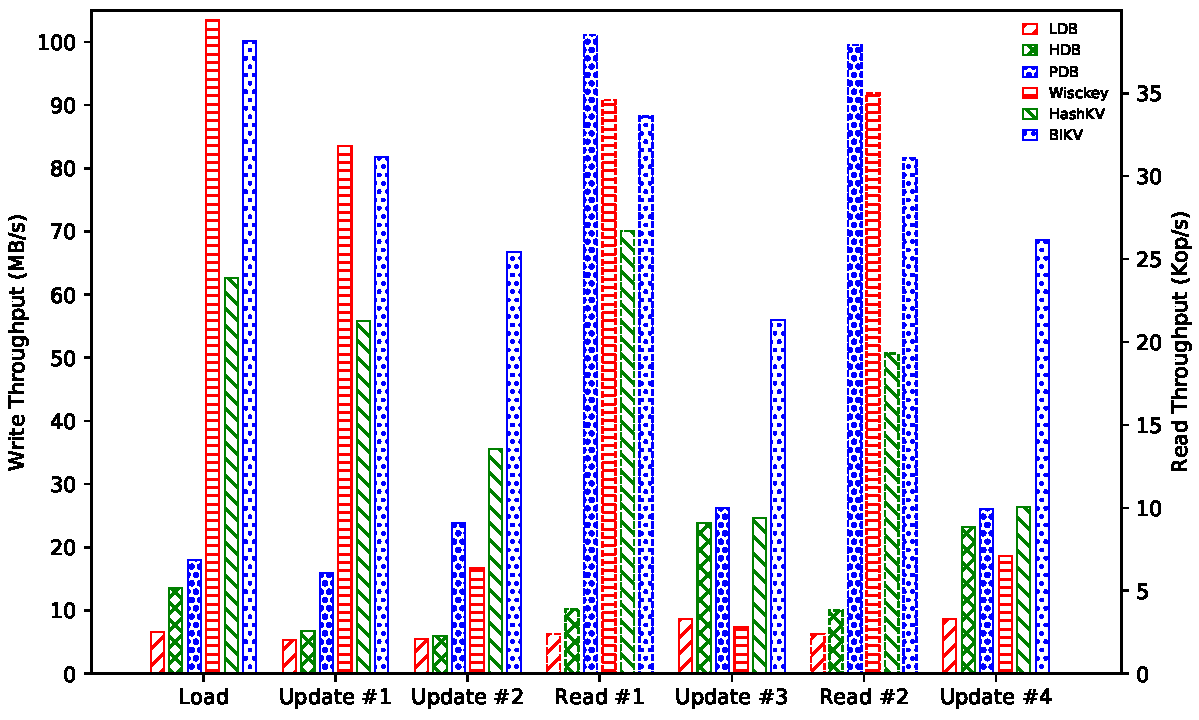
\includegraphics[width=80mm]{total_performance.pdf}
	\caption{The performance of 6 KV stores in 7 steps.}
	\label{fig:pc}
\end{figure}

\subsection{Impact of KV Size}
% 块管理粒床䞺128KBGC阈倌讟计䞺第䞀次update的䞀半从密集GC的角床观察性胜
%KV size蟃小时对于键倌分犻存傚元数据䞎数据倧小接近即LSM-tree䞭的数据key,offset)和vLog䞭的数据keysize,valuesize,key,value)的size盞差倍数䞍倧䜿埗键倌分犻存傚具有明星劣势1.数据需芁写2仜写匀销增加近䞀倍2.空闎匀销倧䞔䌚造成蟃倧的写攟倧键倌分犻存傚比LSM-based存傚圚KV size小时性胜差圓size倧于1KB时性胜奜已经圚其他工䜜䞭埗到证明 \cite{Wisckey, HashKV}。圚这䞀节我们䞻芁观察䞉种键倌分犻存傚对于䞍同KV size的性胜。
We study the performance of KV stores under various KV pair sizes which vary from 256 B to 16 KB. Specifically, we adjust the KV pair size by only changing the value size and keeping the key size fixed at 24 B. We maintain the number of KV pairs loaded or updated to acquire the performance of KV stores under the same order of magnitude operations. We reduce the number of inserts/reads to 10 M and that of updates to 3 M when the KV size is 16 KB because of the limitation of SSD size. Thus, for the KV pair size of 4 KB and 16 KB, the total size of inserts and each round updates is 153 GB and 46 GB, respectively.

We set the capacity of KV separated stores as 45 GB that makes them start to trigger GC in Update \#1. In latter update steps, updates are issued to the fully filled value store and will trigger GC frequently, thus forming a GC-intensive workload. In BIKV, the block size is 128 KB. The experimental results are as shown in Fig.\ref{fig:kv}. We can observe the write/read performance and write amplification under various KV pair sizes. 

%摘自hashKV
%We include both P2 and P3 to ensure that the update performance is stable. HashKV adds a separate region in the value store file for the cold data log.

\begin{figure} [!t]
	\setlength{\abovecaptionskip}{0.cm}	
	\setlength{\belowcaptionskip}{-0.cm}
	\centering
	\subfigure {
		\begin{minipage}{\linewidth}
			\centering
			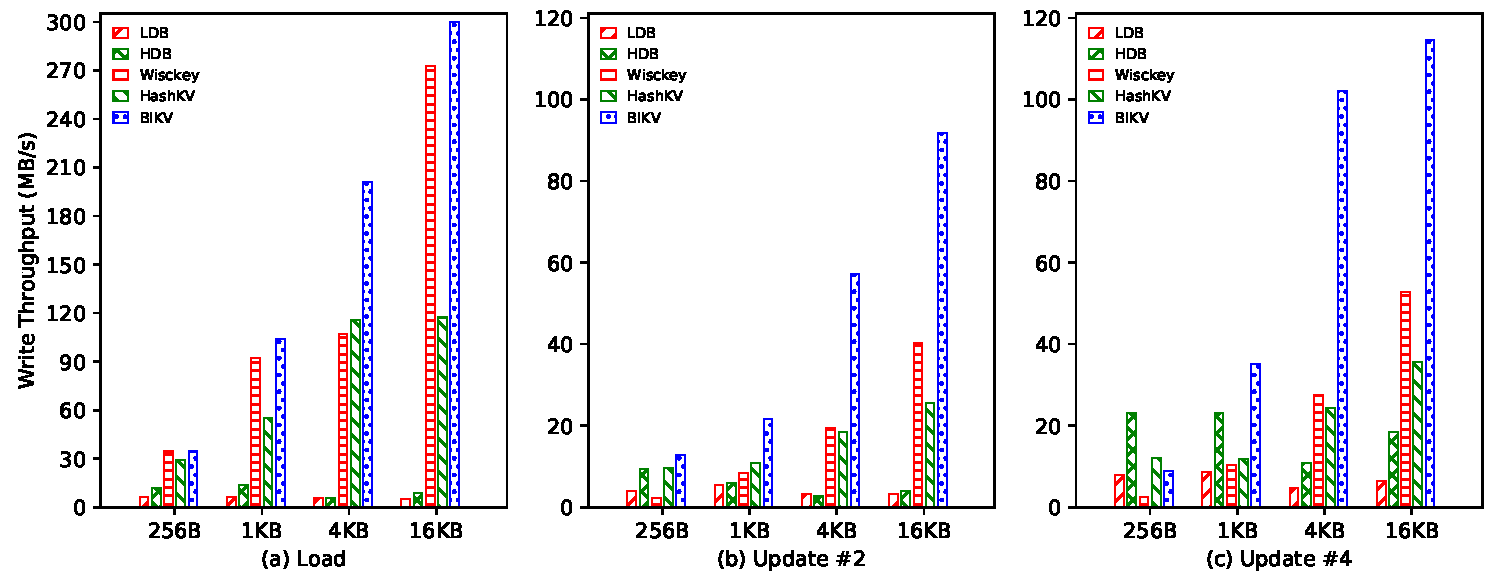
\includegraphics[width=85mm]{kvsize_wt.pdf}
		\end{minipage}
	}  	
	%\vfill
	\subfigure {
		\begin{minipage}[t]{0.31\linewidth}
			\centering
			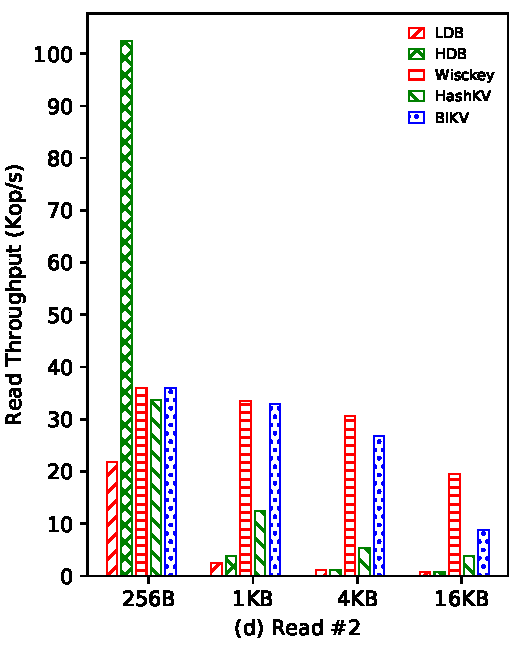
\includegraphics[width=27mm]{kvsize_r.pdf}
		\end{minipage}
		\hfill
		%\vspace{0.02cm}
		\begin{minipage}[t]{0.31\linewidth}
			\centering
			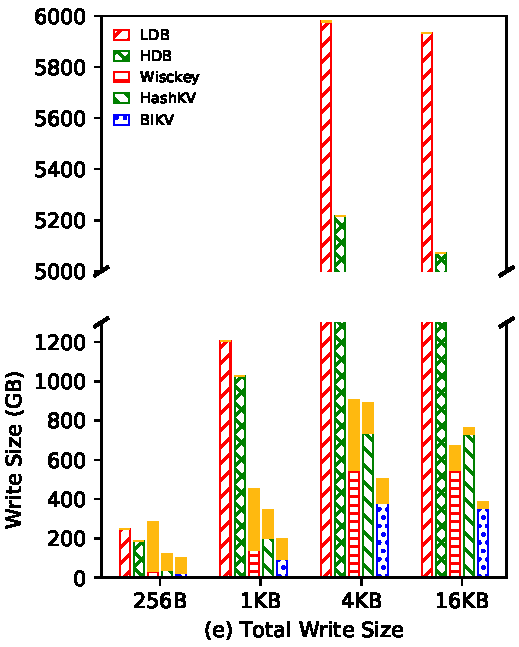
\includegraphics[width=27mm]{kvsize_tw.pdf}
		\end{minipage}
		\hfill
		%\vspace{0.02cm}
		\begin{minipage}[t]{0.31\linewidth}
			\centering
			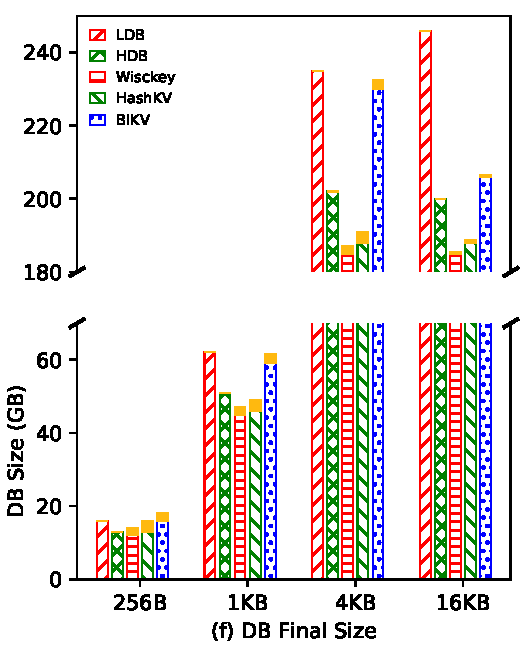
\includegraphics[width=27mm]{kvsize_fs.pdf}
		\end{minipage}
	}
	\caption{Experimental results of 5 KV stores under various KV pair sizes.{\color{red}{why PDB is not tested in these experiments}}}
	\label{fig:kv}
\end{figure}

\paragraph*{Write performance}
%load 和 update2的性胜
We show the write throughput in Load, Update \#2 and Update \#4 of five KV stores under various KV pair size, to illustrate the write performance under random write, intensive GC and intensive update, respectively.

In Load, the write performance of BIKV is always the best, as shown in Fig.\ref{fig:kv} (a), and it is close to Wisckey when KV pair size is less than 1 KB. In Update \#2, the KV separated stores trigger GC intensively. The write performance of BIKV is also the best, as shown in Fig.\ref{fig:kv} (b), benefiting from the lightweight GC. In Update \#4, the write performance of the KV stores is improved, benefiting from {\color{red}{ the numbers of \textit{seek\_compaction} aroused in Read \#2, which clear the space of lower levels.}} {\color{red}{why write would benefit from read?}} . Moreover, up to Update \#4, KV separated stores have accumulated large volume of updates which mitigates GC overhead  in Update \#4, resulting in better write throughput than that in Update \#2, as shown in Fig.\ref{fig:kv} (c).
%It can clearly be seen that the write throughput of the KV stores is better than that in Update #2 at most cases

\paragraph*{Read performance}
We show the read throughput of Read \#2 to illustrate the read performance of the KV stores under various KV pair sizes. As shown in Fig.\ref{fig:kv} (d), when the KV pair size is 256 B, HyperLevelDB has the best read performance because it has less number of SST. The write performance of BIKV approaches that of Wisckey when the size of KV pair is less than 1 KB, and it is worse than Wisckey when the size of KV pair is larger than 4 KB. The reason is due to the large random reads caused by in-place updates.

\paragraph*{Write amplification}
%the difference in write amplification between NG-KV and other stores goes up as the number of keys increases. 
In the KV separated stores, the storage space consists of the key store and value store. We use the solid bar to represent the size of the key store as shown in Fig.\ref{fig:kv} (e) and (f). We combine the size of cold data log and vLog for HashKV. 

The total write size of BIKV is always the least. For KV separated stores, when the KV pair size is less than 1 KB, the total write size of the key store is even larger than that of the value store, as shown in Fig.\ref{fig:kv} (e). The final size of BIKV is close to LevelDB in most cases and is consistently larger than the other three as shown in Fig.\ref{fig:kv} (f), because it appends the valid data left in each GC to BILog. Write amplification (WA) is obtained by dividing the total write size by the total data size, e.g., when KV pair size is 1 KB, the data size of five rounds writes is about 84 GB. WA of LSM structured stores goes up as the KV pair size increases, e.g., it scales from 11.9 to 17.8 X in Wisckey. On the contrary, WA of KV separated stores goes down as the KV pair size increases. WA of BIKV is always the least, which decreases from 4.8 to 1.5 X.

%Corresponding to GC aroused in vLog and compaction aroused in the LSM-tree, we represent the number of GC and compaction in the form of "GC - C" in the column of total write. For HashKV, the cold data size in HashKV is 236MB.

\subsection{Impact of GC Timing}
%3䞪KV分犻的store之闎比蟃观察密集GC和非密集GC的系统性胜
We study the write performance of KV separated stores under various GC timing, i.e., the time to start to trigger GC. We set the capacity of value store as 45 GB and 60 GB to make the systems start to trigger GC in the middle of Update \#1 and late of Update \#2, respectively. The KV pair size is of 1 KB. In BIKV, the block size is 4 KB which agrees with the page size in SSD {\color{red}{(SSD page size is not 4KB !! )}} The experimental results are as shown in Fig.\ref{fig:gc}. We can observe that various GC strategies have different impacts not only on the number of GC and write performance but also on the total write size to the LSM-tree and vLog.

\begin{figure}[!t]
	\setlength{\abovecaptionskip}{0.cm}	
	\setlength{\belowcaptionskip}{-0.cm}
	\centering
	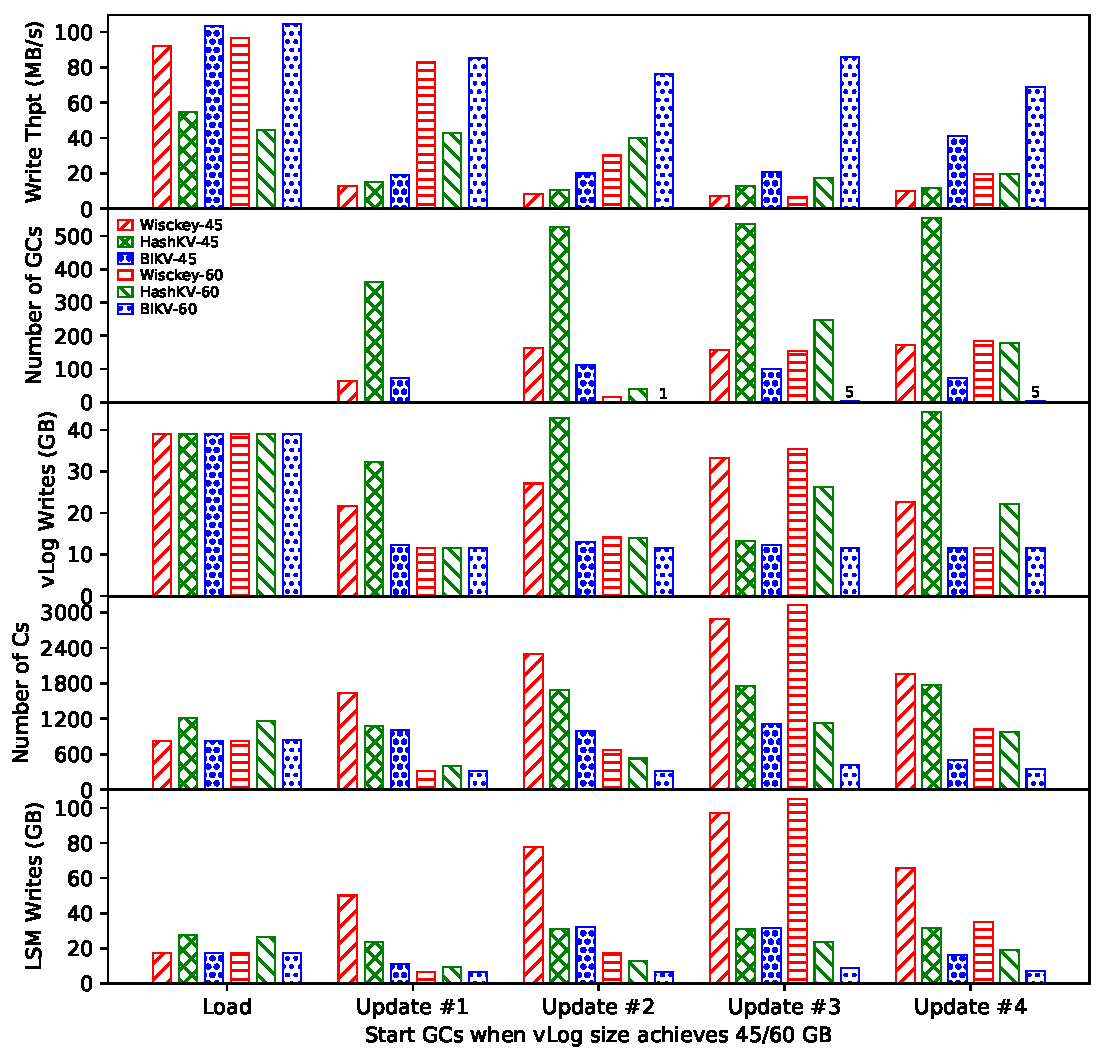
\includegraphics[width=90mm]{gc_timing.pdf}
	\caption{The detailed operations of the key store and value store under different GC timing.}
	\label{fig:gc}
\end{figure}

%密集GC时䞍同的GC策略对LSM产生圱响,compaction数量䞍同写入的数据量䞍同hashkv䞀次GC䞺䞀䞪segment group倧于64MB垊有cold data log
%hashkv因䞺固定size所以产生倧量GC因䞺GC匀销盞对蟃小因歀对写性胜圱响䞍倧
%vlog重写的量倚造成的C和LSM写入就倚写性胜差
%BRKV GC蟃少性胜提升C/LSM/VLOG郜少
For the value store of 45 GB, it forms a GC-intensive workload. When it starts to trigger GC, the write throughput significantly decreases. Various GC strategies result in different amount and sequence of rewritten KV pairs, leading to different number of compaction and total write size in the LSM-tree. For example, in Update \#1, the number of GC in HashKV is the most, resulting in the largest total writes to vLog, but the number of compaction and total write size in the LSM tree is less than Wisckey. For BIKV, the number of GC is a little more than that in Wisckey, but the total writes to vLog, the number of compaction and total writes in the LSM-tree is the least. Generally, BIKV triggers the least GC, which mitigates the impact on write performance and leads to the least total writes to vLog and total writes to the LSM-tree.
%, and the write throughput is better than Wisckey because of the optimized GC

For the value store of 60 GB, before triggering GC frequently, the write throughput of Wisckey and BIKV keeps decreasing from Load to Update \#2. This illustrates that compactions in the LSM-tree have a negative impact on write performance. The total write size and number of compaction in the LSM-tree of HashKV are larger than that of Wisckey and BIKV because of the different sequences of KV pairs writing to vLog. Starting from Update \#3, it triggers GC frequently. BIKV has the best results in all respects, benefiting from the large amount of invalid offsets accumulated under update-intensive workload.


\subsection{Impact of Block Granularity}
%实验参数45GB,1KB实现密集GC块粒床从4KB对霐SSD 页到1MB对霐写buffer以2的倍数增长进行了倧量的实验观察块粒床的圱响
%分析数据发现是块粒床的选择是䞀䞪trade-off块粒床蟃小时䞀䞪块内key数量少容易产生满块䜆是由于GC时䌚选择倱效KV蟃倚的块因歀容易产生倧量随机读而倧粒床块内有效KV蟃倚因歀GC时产生蟃倚的读LSM的操䜜其䞭LSM读操䜜次数圱响曎倚
%给出几䞪块粒床圚U1-U4阶段的写性胜load阶段性胜挖近䌌同时圚衚䞭给出䞀组具有代衚性的实验数据是䞍同块粒床䞋U3阶段的写性胜GC数圚value log䞊进行的读操䜜和LSM䞭进行的查扟操䜜来观察䞍同块粒床对GC及写性胜的圱响。
We study the impact of block granularity on BIKV. The block size varies from 4 KB to 1 MB (aligns to the write buffer). We set the capacity of value store as 45 GB. The KV pair size is of 1 KB. The write throughput of BIKV with various block sizes under four round updates is as shown in Fig.\ref{fig:bg}. We found there exists a trade-off to determine the block size. We illustrate the experimental results in Update \#1 and Update \#3 (as shown in Table \ref{table:bg}) as examples to describe the reasons. \textbf{WT}, \textbf{GCs}, \textbf{BILog-Rs} and \textbf{LSM-Rs} stand for write throughput, the number of GC, the number of read access to BILog and the number of reads in the LSM-tree, respectively.

\begin{figure}[t]
	\setlength{\abovecaptionskip}{0.cm}	
	\setlength{\belowcaptionskip}{-0.cm}
	\centering
	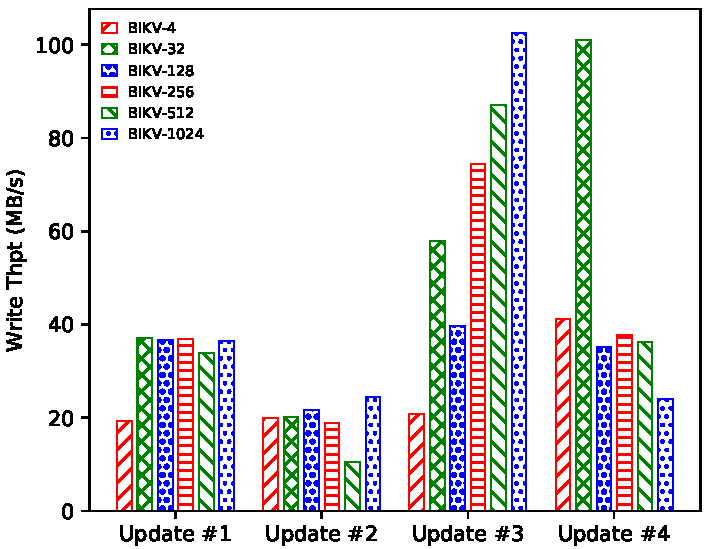
\includegraphics[width=80mm]{block_gra.pdf}
	\makeatletter\def\@captype{figure}\makeatother\caption{Write performance of BIKV under various block sizes.} 
	\label{fig:bg}			
\end{figure}

As shown in Fig. \ref{fig:bg}, the write throughput is relatively stable when the block size of BIKV is 32 KB (32 KB-block). The write performance of 1 MB-block benefits from one write access to BILog when flushing the write buffer. The effect of block size on the write performance of BIKV is not intuitive. Theoretically, smaller block includes less number of KV pairs, thus it is easier to accumulate entirely invalid blocks. However, since BIKV prefers to recycle the invalid blocks with more invalid flags, it would lead to random accesses to BILog in each GC. On the contrary, for the larger block, it is hard to accumulate many invalid Offsets in each block, thus it is more likely to cause a few visits to BILog in each GC. However, it would generate more reads to the LSM-tree because of less invalid flags. In short, the cost of smaller block size is on multiple access to BILog while larger blocks size costs a lot on large amount of random reads to the LSM-tree.

In Update \#1, BIKV starts to trigger GC. The number of GC is 74 under all the block size. The number of read access to BILog and the number of reads to the LSM-tree caused by GC is (1.2 M, 1.9 M) under 4 KB-block and (74, 3.4 M) under other block size, respectively. The difference is nearly (1.2 M, -1.5 M). But the large amount of read accesses to BILog indicate that the recycled blocks are fragmented, and subsequently it generates a similar number of write accesses to BILog when flushing new data. Thus, the difference is converted to about (2.4 M, -1.5 M), resulting in worse write throughput under 4 KB-block, as shown in Fig. \ref{fig:bg}.

Update \#3 is performed after a round of intensive reads, which improves the write performance and accumulates a number of invalid offsets. However, under various block sizes, the GC strategy triggers different block recycling order in the former two rounds of updates, resulting in extremely different number of invalid offsets in Update \#3. In Table \ref{table:bg}, we show the experimental results of write throughput and detailed GC operations in Update \#3 under various block sizes which also verify the above theoretical analysis. When the block size is 4 KB, BIKV produces large number of read accesses to BILog and reads to the LSM-tree in all the GC processes, resulting in the worst write throughput. Comparing the results of 32 KB-block to 128 KB-block, the number of read access to BILog is similar, but the difference in the number of reads in the LSM-tree leads to varying write performance. Due to the significantly small quantity of reads in the LSM-tree, the write performance of three other larger blocks is much better.
\begin{table}[t]
	\setlength{\abovecaptionskip}{0.cm}	
	\setlength{\belowcaptionskip}{-0.cm}
	\centering		
	\makeatletter\def\@captype{table}\makeatother\caption{The detailed GC operations in Update \#3 under various block sizes. }
	\label{table:bg}
	\renewcommand\tabcolsep{4pt}
	\renewcommand\arraystretch{1.1}
	\scalebox{0.8}{			
	\begin{tabular}{ccccccc}
		\toprule
		& {\textbf{4KB}} & \textbf{32KB} & \textbf{128KB} & \textbf{256KB} & \textbf{512KB} & \textbf{1MB} \\
		\midrule
		WT (MB/s) & 20.9 & 57.9 &  39.7 & 74.5 & 87.1 & 102.5  \\
		GCs & 99 & 105 & 120 &  84 & 88 & 123  \\
		BILog-Rs & 1,622,016 & 558 & 546 & 367 & 827 & 270\\
		LSM-Rs & 2,890,235 & 1,477,795 & 3,222,273 & 986,485 & 516,395 & 374,352 \\
		\bottomrule
	\end{tabular}
	}
\end{table} 

\subsection{Disscussion}
%compactionGC对其他KV store的圱响
%原因圚vLog䞭无序䜆是圚LSM-tree䞭有序䜿埗连续的倱效数据可胜无法短时闎内同时被discard劂果觊发GC就需芁额倖的查扟匀销圚LSM-tree䞭通过hash等方法将数据分区同䞀范囎内数据䌚曎快compaction曎快地获埗倱效offset减蜻GC匀销䞍甚再去LSM-tree查扟提高倱效块利甚率
BIKV is implemented atop the design of Wisckey. Besides the memory cost of BIKV, based on the experimental results, we discuss and conclude the differences between BIKV and Wisckey as follows:
\begin{itemize}
	\item BIKV achieves hot and cold data separation by appending the valid data left in GC process to BILog. Thus, the size of BILog is dynamically extended and it is necessary to reserve enough space for expanding;
	\item Based on the experimental results of 7-step mixed workload with the value store size being 45GB, we conclude that:
		\item[-] The write performance of BIKV and Wisckey is similar under write-intensive workload, e.g., Load;
		\item[-] Due to the lightweight GC, BIKV reduces the volume of data rewrites to BILog and the number of reads to the LSM-tree during GC, but meanwhile it causes more accesses to BILog under small block size, e.g., 4 KB block;
		\item[-] BIKV significantly improves write performance and mitigates write amplification under update-intensive workload, e.g., Update \#2;
		\item[-] The in-place updates of BILog has a negative impact on read performance of BIKV, e.g., the read performance under 4 KB KV pair size.
	\item Compactions in the LSM-tree has a negative impact on the write performance of BIKV and Wisckey. It is better to use optimized LSM-tree as the key store.
	\item We did not evaluate the performance of the range query because the unchanged LSM-tree, as well as the random read performance and parallelism characteristics of SSD, lead to stable performance of range query, as verified by the results in HashKV \cite{HashKV}.
\end{itemize}

\section{Related Work} \label{related}
%LSM-tree的compaction读性胜等䌘化的工䜜䞎本工䜜正亀䞔有利于KV分犻的工䜜
LSM-tree \cite{LSMtree} is a popular structure for write-intensive workloads in the persistent key-value stores. Much work has gone into optimizing the LSM-tree for write amplification ~\cite{VTtree,TRIAD,PebblesDB}, write performance \cite{RocksDB,FloDB,cLSM} and various storage medias \cite{LOCS,SlimDB,NoveLSM}. The data organization of them can be divided into a multi-level log structure and KV separation.
%multi-leveled log structure
%Most of them maintain the multi-leveled log-structured merging data organization, while others are KV separated \cite{Wisckey,HashKV}. 

\textbf{Multi-level log structure:} HyperlevelDB \cite{HyperLevelDB} makes flushing concurrent with compaction to increase write throughput. RocksDB \cite{RocksDB} introduces multi-threaded compaction and tackles other concurrency issues upon LevelDB \cite{LevelDB}. bLSM \cite{bLSM} introduces a new merge scheduler to minimize write latency and reduce its negative impact on write performance. VT-tree \cite{VTtree} avoids unnecessary data copying for data that is already sorted using an extra level of indirection. cLSM \cite{cLSM} introduces a new algorithm for increasing concurrency with a goal of increasing scalability. LSM-trie \cite{LSMtrie} combines hash and trie-tree to organize KV pairs, proposes an efficient compaction strategy and builds stronger Bloom filters for fast searches on disk, but gives up range queries. FloDB \cite{FloDB} inserts an additional fast in-memory buffer on top of Memtable to achieve better write performance. Yue et al. \cite{skiptree} proposes a skip-tree to push KV pairs to non-adjacent, larger-capacity levels to reduce the data traffic from the write buffer to bottom level. TRIAD \cite{TRIAD} uses a holistic combination of the optimizations at the memory component level, the storage level and the commit log level to improve the throughput by reducing the write amplification. PebblesDB \cite{PebblesDB} proposes a new data structure FLSM with the notion of guards, and avoids rewriting data in the same level to reduce write amplification. Mei et al. \cite{LDS} implements an direct storage system based on LevelDB to fully utilize the LSM-tree features and provide high write performance. LOCS\cite{LOCS} exposes internal flash channels and improves LSM compaction by exploiting the internal parallelism of open-channel SSDs. SlimDB \cite{SlimDB} introduces a space-efficient semi-sorting storage, combined with the Cuckoo filter and an slection model for index and filter to improve read and write performance for SSD. NoveLSM \cite{NoveLSM} utilizes the NVM features to redesign LSM for NVM by implementing byte-addressable skiplist, direct mutability of persistent state, and opportunistic read parallelism. SEALDB \cite{SEALDB} collects and groups participating data of each compaction into sets and creates dynamic bands to eliminate write amplification for SMR drives. {\color{red}{SILK \cite{SILK} figures out that the high tail latency of the LSM structured stores is caused by the interference between client writes, flushes as well as compactions, and introduces an I/O scheduler to manage external client load and internal LSM maintenance work.}}

\textbf{KV separation:} WiscKey \cite{Wisckey} separates keys from values and only stores keys in the LSM-tree to significantly reduce the write amplification caused by compaction for SSD and utilizes the random performance and parallelism characteristics of SSD to provide efficient read and range query performance. HashKV \cite{HashKV} builds hash-based data grouping to deterministically map values to storage space atop KV separation, to make GC efficient and provide high write performance under update-intensive workloads. {\color{red}{KVell \cite{KVell} aims to reduce CPU-overhead and utilize modern NVMe SSDs at maximum bandwidth by relying on a share-nothing architecture, using one in-memory B tree per worker to store the location of KV pairs which are stored out of order in various slabs on disk according to their sizes. KVell reclaims space with the free lists which contain the locations of deleted KV pairs. Freed locations are reused when new data comes.}}

BIKV also builds on KV separation and takes one step further to address efficient storage space reclaiming in the presence of intensive triggers. {\color{red}{The design of GC in KVell is similar to a GC method we used to take into consideration ( Section \ref{bd}), that is buffering the offsets of the KV pairs discarded in the LSM-tree, and reusing them when flushing new data. But, this method would result in a large number of costly system calls. To remedy this problem, we build a block manager to assist reclaiming space and reuse the freed space in blocks.}} The above KV stores and BIKV are stand-alone KV stores that can serve as the foundation of distributed storage systems (e.g., Cassandra \cite{ Cassandra}, Dynamo \cite{ Dynamo}, and HBase \cite{HBase}). The studies for LSM optimization are orthogonal to KV separated stores, especially those who focus on improving the write performance and read performance, which can be leveraged in synergy to KV separated stores to enhance I/O efficiency further.

\section{Conclusion} \label{conclusion}

% investigate variable size kvs
% overhead analysis 
% reference 21
This paper presents BIKV which consists of a key store, a block manager and a value store, enabling efficient storage space reclaiming which leads to improvement on write performance and write amplification under GC-intensive workloads. The block manager gathers invalid offsets from the discarded KV pairs in the LSM-tree and assists block recycling during the GC process in the vLog. Based on the block manager, BIKV transforms the vLog from a conventional circular log to BILog, a block-conscious in-place update log. BIKV realizes hot/cold data separation to avoid relocating cold data during GC process by dividing BILog into main space (for new data) and reserved space (for the valid data left in GC). Experimental results show that BIKV achieves high write throughput and mitigates write amplification under GC-intensive workloads with a moderate cost of memory space for the block manager. Memory cost of the block manager mainly consists of two state bitmaps and three block buffers, for example, if BILog accommodates 40 M KV pairs, and the total number of blocks in the three buffers is 150,000, the memory cost is only about 11 MB. We plan to expand BIKV to support varying key value sizes in our future work. 
%BIKV improves write performance and write amplification under GC-intensive workloads with the cost of memory space for the block manager, which is about 43 MB for 40 M KV pairs.

\iffalse
\begin{acks}
	...
\end{acks}
\fi

%\begin{thebibliography}{00}

%\end{thebibliography}
\bibliographystyle{ACM-Reference-Format}
\bibliography{bikv}
%\vspace{12pt}


\end{document}
